\documentclass[tikz,border=6pt]{standalone}
\usepackage{lmodern}
\usepackage[T1]{fontenc}
\usepackage{amssymb}
\usetikzlibrary{arrows.meta}
\definecolor{okgreen}{RGB}{0,158,115}
\definecolor{okverm}{RGB}{213,94,0}
\begin{document}
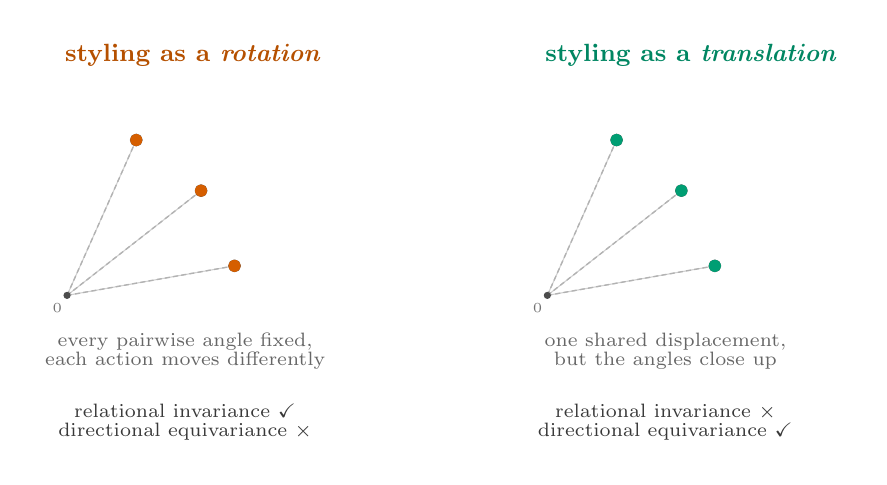
\begin{tikzpicture}[font=\small,line cap=round,line join=round,x=1cm,y=1cm]
\useasboundingbox (-0.5,-2.05) rectangle (10.05,3.4);
\begin{scope}[shift={(0.0,0)}]
\node[font=\small\bfseries,text=okverm!85!black,anchor=west] at (-0.15,3.05) {styling as a \emph{rotation}};
\draw[black!18,line width=0.4pt] (0,0) -- (2.127,0.375);
\draw[black!30,line width=0.5pt,dash pattern=on 1.6pt off 1.4pt] (0,0) -- (2.127,0.375);
\node[circle,draw=black!65,fill=white,inner sep=0pt,minimum size=4pt,line width=0.6pt] at (2.127,0.375) {};
\node[circle,fill=okverm,inner sep=0pt,minimum size=4.4pt] at (2.127,0.375) {};
\draw[black!18,line width=0.4pt] (0,0) -- (1.702,1.330);
\draw[black!30,line width=0.5pt,dash pattern=on 1.6pt off 1.4pt] (0,0) -- (1.702,1.330);
\node[circle,draw=black!65,fill=white,inner sep=0pt,minimum size=4pt,line width=0.6pt] at (1.702,1.330) {};
\node[circle,fill=okverm,inner sep=0pt,minimum size=4.4pt] at (1.702,1.330) {};
\draw[black!18,line width=0.4pt] (0,0) -- (0.879,1.973);
\draw[black!30,line width=0.5pt,dash pattern=on 1.6pt off 1.4pt] (0,0) -- (0.879,1.973);
\node[circle,draw=black!65,fill=white,inner sep=0pt,minimum size=4pt,line width=0.6pt] at (0.879,1.973) {};
\node[circle,fill=okverm,inner sep=0pt,minimum size=4.4pt] at (0.879,1.973) {};
\fill[black!70] (0,0) circle (1.3pt);
\node[font=\tiny,text=black!55,anchor=north east] at (0.06,0.02) {$0$};
\node[font=\scriptsize,text=black!60,align=center,anchor=north] at (1.5,-0.35) {every pairwise angle fixed,\\[-1pt] each action moves differently};
\node[font=\scriptsize,text=black!78,align=center,anchor=north] at (1.5,-1.25) {relational invariance \checkmark\\[-1pt] directional equivariance $\times$};
\end{scope}
\begin{scope}[shift={(6.1,0)}]
\node[font=\small\bfseries,text=okgreen!85!black,anchor=west] at (-0.15,3.05) {styling as a \emph{translation}};
\draw[black!18,line width=0.4pt] (0,0) -- (2.127,0.375);
\draw[black!30,line width=0.5pt,dash pattern=on 1.6pt off 1.4pt] (0,0) -- (2.127,0.375);
\node[circle,draw=black!65,fill=white,inner sep=0pt,minimum size=4pt,line width=0.6pt] at (2.127,0.375) {};
\node[circle,fill=okgreen,inner sep=0pt,minimum size=4.4pt] at (2.127,0.375) {};
\draw[black!18,line width=0.4pt] (0,0) -- (1.702,1.330);
\draw[black!30,line width=0.5pt,dash pattern=on 1.6pt off 1.4pt] (0,0) -- (1.702,1.330);
\node[circle,draw=black!65,fill=white,inner sep=0pt,minimum size=4pt,line width=0.6pt] at (1.702,1.330) {};
\node[circle,fill=okgreen,inner sep=0pt,minimum size=4.4pt] at (1.702,1.330) {};
\draw[black!18,line width=0.4pt] (0,0) -- (0.879,1.973);
\draw[black!30,line width=0.5pt,dash pattern=on 1.6pt off 1.4pt] (0,0) -- (0.879,1.973);
\node[circle,draw=black!65,fill=white,inner sep=0pt,minimum size=4pt,line width=0.6pt] at (0.879,1.973) {};
\node[circle,fill=okgreen,inner sep=0pt,minimum size=4.4pt] at (0.879,1.973) {};
\fill[black!70] (0,0) circle (1.3pt);
\node[font=\tiny,text=black!55,anchor=north east] at (0.06,0.02) {$0$};
\node[font=\scriptsize,text=black!60,align=center,anchor=north] at (1.5,-0.35) {one shared displacement,\\[-1pt] but the angles close up};
\node[font=\scriptsize,text=black!78,align=center,anchor=north] at (1.5,-1.25) {relational invariance $\times$\\[-1pt] directional equivariance \checkmark};
\end{scope}
\end{tikzpicture}
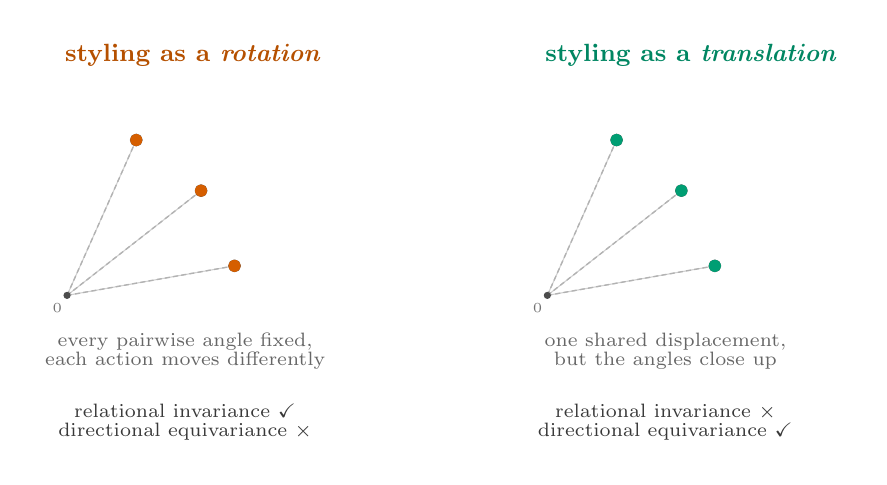
\begin{tikzpicture}[font=\small,line cap=round,line join=round,x=1cm,y=1cm]
\useasboundingbox (-0.5,-2.05) rectangle (10.05,3.4);
\begin{scope}[shift={(0.0,0)}]
\node[font=\small\bfseries,text=okverm!85!black,anchor=west] at (-0.15,3.05) {styling as a \emph{rotation}};
\draw[black!18,line width=0.4pt] (0,0) -- (2.127,0.375);
\draw[black!30,line width=0.5pt,dash pattern=on 1.6pt off 1.4pt] (0,0) -- (2.127,0.375);
\node[circle,draw=black!65,fill=white,inner sep=0pt,minimum size=4pt,line width=0.6pt] at (2.127,0.375) {};
\node[circle,fill=okverm,inner sep=0pt,minimum size=4.4pt] at (2.127,0.375) {};
\draw[black!18,line width=0.4pt] (0,0) -- (1.702,1.330);
\draw[black!30,line width=0.5pt,dash pattern=on 1.6pt off 1.4pt] (0,0) -- (1.702,1.330);
\node[circle,draw=black!65,fill=white,inner sep=0pt,minimum size=4pt,line width=0.6pt] at (1.702,1.330) {};
\node[circle,fill=okverm,inner sep=0pt,minimum size=4.4pt] at (1.702,1.330) {};
\draw[black!18,line width=0.4pt] (0,0) -- (0.879,1.973);
\draw[black!30,line width=0.5pt,dash pattern=on 1.6pt off 1.4pt] (0,0) -- (0.879,1.973);
\node[circle,draw=black!65,fill=white,inner sep=0pt,minimum size=4pt,line width=0.6pt] at (0.879,1.973) {};
\node[circle,fill=okverm,inner sep=0pt,minimum size=4.4pt] at (0.879,1.973) {};
\fill[black!70] (0,0) circle (1.3pt);
\node[font=\tiny,text=black!55,anchor=north east] at (0.06,0.02) {$0$};
\node[font=\scriptsize,text=black!60,align=center,anchor=north] at (1.5,-0.35) {every pairwise angle fixed,\\[-1pt] each action moves differently};
\node[font=\scriptsize,text=black!78,align=center,anchor=north] at (1.5,-1.25) {relational invariance \checkmark\\[-1pt] directional equivariance $\times$};
\end{scope}
\begin{scope}[shift={(6.1,0)}]
\node[font=\small\bfseries,text=okgreen!85!black,anchor=west] at (-0.15,3.05) {styling as a \emph{translation}};
\draw[black!18,line width=0.4pt] (0,0) -- (2.127,0.375);
\draw[black!30,line width=0.5pt,dash pattern=on 1.6pt off 1.4pt] (0,0) -- (2.127,0.375);
\node[circle,draw=black!65,fill=white,inner sep=0pt,minimum size=4pt,line width=0.6pt] at (2.127,0.375) {};
\node[circle,fill=okgreen,inner sep=0pt,minimum size=4.4pt] at (2.127,0.375) {};
\draw[black!18,line width=0.4pt] (0,0) -- (1.702,1.330);
\draw[black!30,line width=0.5pt,dash pattern=on 1.6pt off 1.4pt] (0,0) -- (1.702,1.330);
\node[circle,draw=black!65,fill=white,inner sep=0pt,minimum size=4pt,line width=0.6pt] at (1.702,1.330) {};
\node[circle,fill=okgreen,inner sep=0pt,minimum size=4.4pt] at (1.702,1.330) {};
\draw[black!18,line width=0.4pt] (0,0) -- (0.879,1.973);
\draw[black!30,line width=0.5pt,dash pattern=on 1.6pt off 1.4pt] (0,0) -- (0.879,1.973);
\node[circle,draw=black!65,fill=white,inner sep=0pt,minimum size=4pt,line width=0.6pt] at (0.879,1.973) {};
\node[circle,fill=okgreen,inner sep=0pt,minimum size=4.4pt] at (0.879,1.973) {};
\fill[black!70] (0,0) circle (1.3pt);
\node[font=\tiny,text=black!55,anchor=north east] at (0.06,0.02) {$0$};
\node[font=\scriptsize,text=black!60,align=center,anchor=north] at (1.5,-0.35) {one shared displacement,\\[-1pt] but the angles close up};
\node[font=\scriptsize,text=black!78,align=center,anchor=north] at (1.5,-1.25) {relational invariance $\times$\\[-1pt] directional equivariance \checkmark};
\end{scope}
\end{tikzpicture}
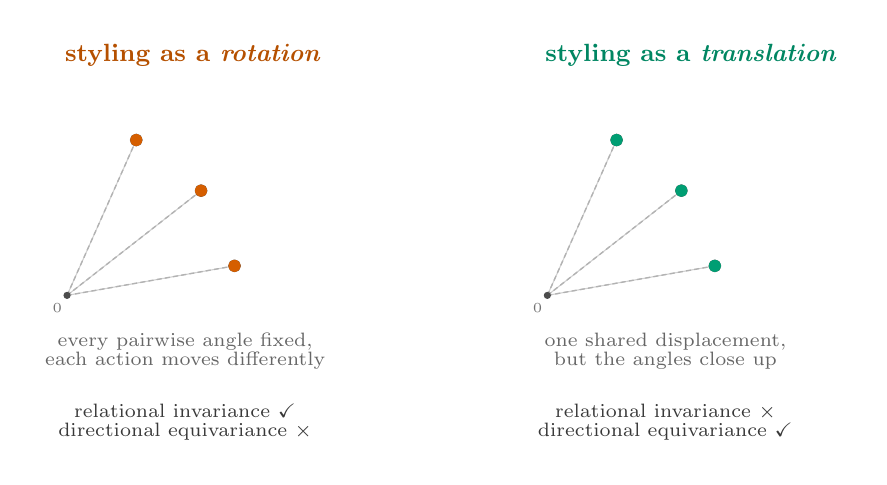
\begin{tikzpicture}[font=\small,line cap=round,line join=round,x=1cm,y=1cm]
\useasboundingbox (-0.5,-2.05) rectangle (10.05,3.4);
\begin{scope}[shift={(0.0,0)}]
\node[font=\small\bfseries,text=okverm!85!black,anchor=west] at (-0.15,3.05) {styling as a \emph{rotation}};
\draw[black!18,line width=0.4pt] (0,0) -- (2.127,0.375);
\draw[black!30,line width=0.5pt,dash pattern=on 1.6pt off 1.4pt] (0,0) -- (2.127,0.375);
\node[circle,draw=black!65,fill=white,inner sep=0pt,minimum size=4pt,line width=0.6pt] at (2.127,0.375) {};
\node[circle,fill=okverm,inner sep=0pt,minimum size=4.4pt] at (2.127,0.375) {};
\draw[black!18,line width=0.4pt] (0,0) -- (1.702,1.330);
\draw[black!30,line width=0.5pt,dash pattern=on 1.6pt off 1.4pt] (0,0) -- (1.702,1.330);
\node[circle,draw=black!65,fill=white,inner sep=0pt,minimum size=4pt,line width=0.6pt] at (1.702,1.330) {};
\node[circle,fill=okverm,inner sep=0pt,minimum size=4.4pt] at (1.702,1.330) {};
\draw[black!18,line width=0.4pt] (0,0) -- (0.879,1.973);
\draw[black!30,line width=0.5pt,dash pattern=on 1.6pt off 1.4pt] (0,0) -- (0.879,1.973);
\node[circle,draw=black!65,fill=white,inner sep=0pt,minimum size=4pt,line width=0.6pt] at (0.879,1.973) {};
\node[circle,fill=okverm,inner sep=0pt,minimum size=4.4pt] at (0.879,1.973) {};
\fill[black!70] (0,0) circle (1.3pt);
\node[font=\tiny,text=black!55,anchor=north east] at (0.06,0.02) {$0$};
\node[font=\scriptsize,text=black!60,align=center,anchor=north] at (1.5,-0.35) {every pairwise angle fixed,\\[-1pt] each action moves differently};
\node[font=\scriptsize,text=black!78,align=center,anchor=north] at (1.5,-1.25) {relational invariance \checkmark\\[-1pt] directional equivariance $\times$};
\end{scope}
\begin{scope}[shift={(6.1,0)}]
\node[font=\small\bfseries,text=okgreen!85!black,anchor=west] at (-0.15,3.05) {styling as a \emph{translation}};
\draw[black!18,line width=0.4pt] (0,0) -- (2.127,0.375);
\draw[black!30,line width=0.5pt,dash pattern=on 1.6pt off 1.4pt] (0,0) -- (2.127,0.375);
\node[circle,draw=black!65,fill=white,inner sep=0pt,minimum size=4pt,line width=0.6pt] at (2.127,0.375) {};
\node[circle,fill=okgreen,inner sep=0pt,minimum size=4.4pt] at (2.127,0.375) {};
\draw[black!18,line width=0.4pt] (0,0) -- (1.702,1.330);
\draw[black!30,line width=0.5pt,dash pattern=on 1.6pt off 1.4pt] (0,0) -- (1.702,1.330);
\node[circle,draw=black!65,fill=white,inner sep=0pt,minimum size=4pt,line width=0.6pt] at (1.702,1.330) {};
\node[circle,fill=okgreen,inner sep=0pt,minimum size=4.4pt] at (1.702,1.330) {};
\draw[black!18,line width=0.4pt] (0,0) -- (0.879,1.973);
\draw[black!30,line width=0.5pt,dash pattern=on 1.6pt off 1.4pt] (0,0) -- (0.879,1.973);
\node[circle,draw=black!65,fill=white,inner sep=0pt,minimum size=4pt,line width=0.6pt] at (0.879,1.973) {};
\node[circle,fill=okgreen,inner sep=0pt,minimum size=4.4pt] at (0.879,1.973) {};
\fill[black!70] (0,0) circle (1.3pt);
\node[font=\tiny,text=black!55,anchor=north east] at (0.06,0.02) {$0$};
\node[font=\scriptsize,text=black!60,align=center,anchor=north] at (1.5,-0.35) {one shared displacement,\\[-1pt] but the angles close up};
\node[font=\scriptsize,text=black!78,align=center,anchor=north] at (1.5,-1.25) {relational invariance $\times$\\[-1pt] directional equivariance \checkmark};
\end{scope}
\end{tikzpicture}
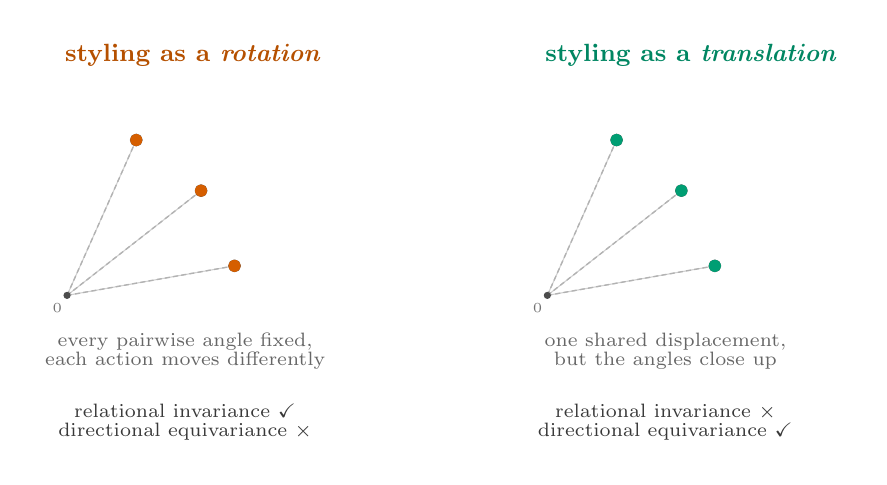
\begin{tikzpicture}[font=\small,line cap=round,line join=round,x=1cm,y=1cm]
\useasboundingbox (-0.5,-2.05) rectangle (10.05,3.4);
\begin{scope}[shift={(0.0,0)}]
\node[font=\small\bfseries,text=okverm!85!black,anchor=west] at (-0.15,3.05) {styling as a \emph{rotation}};
\draw[black!18,line width=0.4pt] (0,0) -- (2.127,0.375);
\draw[black!30,line width=0.5pt,dash pattern=on 1.6pt off 1.4pt] (0,0) -- (2.127,0.375);
\node[circle,draw=black!65,fill=white,inner sep=0pt,minimum size=4pt,line width=0.6pt] at (2.127,0.375) {};
\node[circle,fill=okverm,inner sep=0pt,minimum size=4.4pt] at (2.127,0.375) {};
\draw[black!18,line width=0.4pt] (0,0) -- (1.702,1.330);
\draw[black!30,line width=0.5pt,dash pattern=on 1.6pt off 1.4pt] (0,0) -- (1.702,1.330);
\node[circle,draw=black!65,fill=white,inner sep=0pt,minimum size=4pt,line width=0.6pt] at (1.702,1.330) {};
\node[circle,fill=okverm,inner sep=0pt,minimum size=4.4pt] at (1.702,1.330) {};
\draw[black!18,line width=0.4pt] (0,0) -- (0.879,1.973);
\draw[black!30,line width=0.5pt,dash pattern=on 1.6pt off 1.4pt] (0,0) -- (0.879,1.973);
\node[circle,draw=black!65,fill=white,inner sep=0pt,minimum size=4pt,line width=0.6pt] at (0.879,1.973) {};
\node[circle,fill=okverm,inner sep=0pt,minimum size=4.4pt] at (0.879,1.973) {};
\fill[black!70] (0,0) circle (1.3pt);
\node[font=\tiny,text=black!55,anchor=north east] at (0.06,0.02) {$0$};
\node[font=\scriptsize,text=black!60,align=center,anchor=north] at (1.5,-0.35) {every pairwise angle fixed,\\[-1pt] each action moves differently};
\node[font=\scriptsize,text=black!78,align=center,anchor=north] at (1.5,-1.25) {relational invariance \checkmark\\[-1pt] directional equivariance $\times$};
\end{scope}
\begin{scope}[shift={(6.1,0)}]
\node[font=\small\bfseries,text=okgreen!85!black,anchor=west] at (-0.15,3.05) {styling as a \emph{translation}};
\draw[black!18,line width=0.4pt] (0,0) -- (2.127,0.375);
\draw[black!30,line width=0.5pt,dash pattern=on 1.6pt off 1.4pt] (0,0) -- (2.127,0.375);
\node[circle,draw=black!65,fill=white,inner sep=0pt,minimum size=4pt,line width=0.6pt] at (2.127,0.375) {};
\node[circle,fill=okgreen,inner sep=0pt,minimum size=4.4pt] at (2.127,0.375) {};
\draw[black!18,line width=0.4pt] (0,0) -- (1.702,1.330);
\draw[black!30,line width=0.5pt,dash pattern=on 1.6pt off 1.4pt] (0,0) -- (1.702,1.330);
\node[circle,draw=black!65,fill=white,inner sep=0pt,minimum size=4pt,line width=0.6pt] at (1.702,1.330) {};
\node[circle,fill=okgreen,inner sep=0pt,minimum size=4.4pt] at (1.702,1.330) {};
\draw[black!18,line width=0.4pt] (0,0) -- (0.879,1.973);
\draw[black!30,line width=0.5pt,dash pattern=on 1.6pt off 1.4pt] (0,0) -- (0.879,1.973);
\node[circle,draw=black!65,fill=white,inner sep=0pt,minimum size=4pt,line width=0.6pt] at (0.879,1.973) {};
\node[circle,fill=okgreen,inner sep=0pt,minimum size=4.4pt] at (0.879,1.973) {};
\fill[black!70] (0,0) circle (1.3pt);
\node[font=\tiny,text=black!55,anchor=north east] at (0.06,0.02) {$0$};
\node[font=\scriptsize,text=black!60,align=center,anchor=north] at (1.5,-0.35) {one shared displacement,\\[-1pt] but the angles close up};
\node[font=\scriptsize,text=black!78,align=center,anchor=north] at (1.5,-1.25) {relational invariance $\times$\\[-1pt] directional equivariance \checkmark};
\end{scope}
\end{tikzpicture}
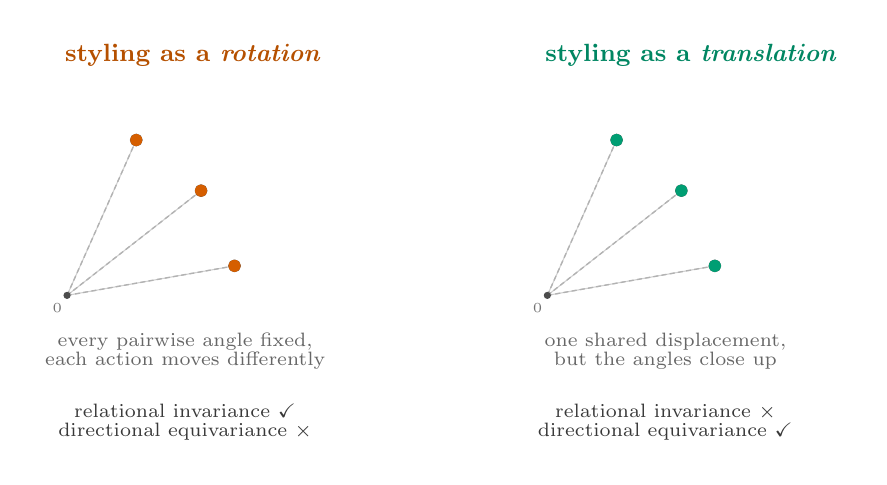
\begin{tikzpicture}[font=\small,line cap=round,line join=round,x=1cm,y=1cm]
\useasboundingbox (-0.5,-2.05) rectangle (10.05,3.4);
\begin{scope}[shift={(0.0,0)}]
\node[font=\small\bfseries,text=okverm!85!black,anchor=west] at (-0.15,3.05) {styling as a \emph{rotation}};
\draw[black!18,line width=0.4pt] (0,0) -- (2.127,0.375);
\draw[black!30,line width=0.5pt,dash pattern=on 1.6pt off 1.4pt] (0,0) -- (2.127,0.375);
\node[circle,draw=black!65,fill=white,inner sep=0pt,minimum size=4pt,line width=0.6pt] at (2.127,0.375) {};
\node[circle,fill=okverm,inner sep=0pt,minimum size=4.4pt] at (2.127,0.375) {};
\draw[black!18,line width=0.4pt] (0,0) -- (1.702,1.330);
\draw[black!30,line width=0.5pt,dash pattern=on 1.6pt off 1.4pt] (0,0) -- (1.702,1.330);
\node[circle,draw=black!65,fill=white,inner sep=0pt,minimum size=4pt,line width=0.6pt] at (1.702,1.330) {};
\node[circle,fill=okverm,inner sep=0pt,minimum size=4.4pt] at (1.702,1.330) {};
\draw[black!18,line width=0.4pt] (0,0) -- (0.879,1.973);
\draw[black!30,line width=0.5pt,dash pattern=on 1.6pt off 1.4pt] (0,0) -- (0.879,1.973);
\node[circle,draw=black!65,fill=white,inner sep=0pt,minimum size=4pt,line width=0.6pt] at (0.879,1.973) {};
\node[circle,fill=okverm,inner sep=0pt,minimum size=4.4pt] at (0.879,1.973) {};
\fill[black!70] (0,0) circle (1.3pt);
\node[font=\tiny,text=black!55,anchor=north east] at (0.06,0.02) {$0$};
\node[font=\scriptsize,text=black!60,align=center,anchor=north] at (1.5,-0.35) {every pairwise angle fixed,\\[-1pt] each action moves differently};
\node[font=\scriptsize,text=black!78,align=center,anchor=north] at (1.5,-1.25) {relational invariance \checkmark\\[-1pt] directional equivariance $\times$};
\end{scope}
\begin{scope}[shift={(6.1,0)}]
\node[font=\small\bfseries,text=okgreen!85!black,anchor=west] at (-0.15,3.05) {styling as a \emph{translation}};
\draw[black!18,line width=0.4pt] (0,0) -- (2.127,0.375);
\draw[black!30,line width=0.5pt,dash pattern=on 1.6pt off 1.4pt] (0,0) -- (2.127,0.375);
\node[circle,draw=black!65,fill=white,inner sep=0pt,minimum size=4pt,line width=0.6pt] at (2.127,0.375) {};
\node[circle,fill=okgreen,inner sep=0pt,minimum size=4.4pt] at (2.127,0.375) {};
\draw[black!18,line width=0.4pt] (0,0) -- (1.702,1.330);
\draw[black!30,line width=0.5pt,dash pattern=on 1.6pt off 1.4pt] (0,0) -- (1.702,1.330);
\node[circle,draw=black!65,fill=white,inner sep=0pt,minimum size=4pt,line width=0.6pt] at (1.702,1.330) {};
\node[circle,fill=okgreen,inner sep=0pt,minimum size=4.4pt] at (1.702,1.330) {};
\draw[black!18,line width=0.4pt] (0,0) -- (0.879,1.973);
\draw[black!30,line width=0.5pt,dash pattern=on 1.6pt off 1.4pt] (0,0) -- (0.879,1.973);
\node[circle,draw=black!65,fill=white,inner sep=0pt,minimum size=4pt,line width=0.6pt] at (0.879,1.973) {};
\node[circle,fill=okgreen,inner sep=0pt,minimum size=4.4pt] at (0.879,1.973) {};
\fill[black!70] (0,0) circle (1.3pt);
\node[font=\tiny,text=black!55,anchor=north east] at (0.06,0.02) {$0$};
\node[font=\scriptsize,text=black!60,align=center,anchor=north] at (1.5,-0.35) {one shared displacement,\\[-1pt] but the angles close up};
\node[font=\scriptsize,text=black!78,align=center,anchor=north] at (1.5,-1.25) {relational invariance $\times$\\[-1pt] directional equivariance \checkmark};
\end{scope}
\end{tikzpicture}
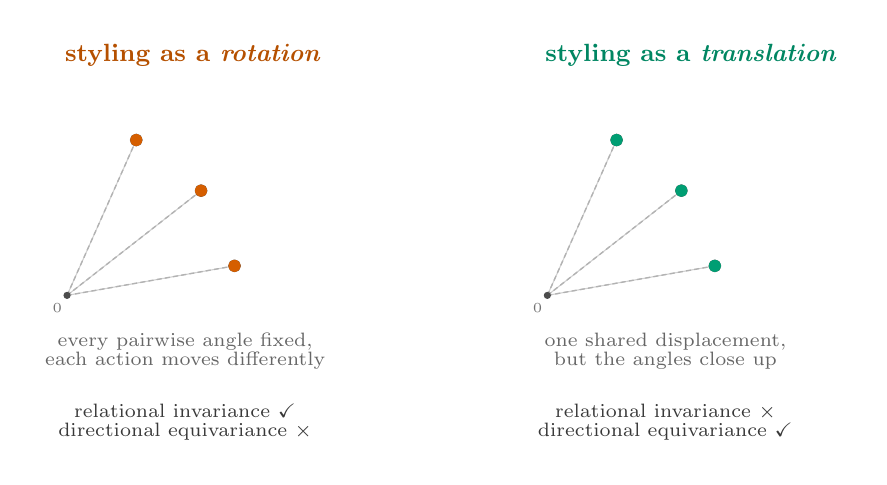
\begin{tikzpicture}[font=\small,line cap=round,line join=round,x=1cm,y=1cm]
\useasboundingbox (-0.5,-2.05) rectangle (10.05,3.4);
\begin{scope}[shift={(0.0,0)}]
\node[font=\small\bfseries,text=okverm!85!black,anchor=west] at (-0.15,3.05) {styling as a \emph{rotation}};
\draw[black!18,line width=0.4pt] (0,0) -- (2.127,0.375);
\draw[black!30,line width=0.5pt,dash pattern=on 1.6pt off 1.4pt] (0,0) -- (2.127,0.375);
\node[circle,draw=black!65,fill=white,inner sep=0pt,minimum size=4pt,line width=0.6pt] at (2.127,0.375) {};
\node[circle,fill=okverm,inner sep=0pt,minimum size=4.4pt] at (2.127,0.375) {};
\draw[black!18,line width=0.4pt] (0,0) -- (1.702,1.330);
\draw[black!30,line width=0.5pt,dash pattern=on 1.6pt off 1.4pt] (0,0) -- (1.702,1.330);
\node[circle,draw=black!65,fill=white,inner sep=0pt,minimum size=4pt,line width=0.6pt] at (1.702,1.330) {};
\node[circle,fill=okverm,inner sep=0pt,minimum size=4.4pt] at (1.702,1.330) {};
\draw[black!18,line width=0.4pt] (0,0) -- (0.879,1.973);
\draw[black!30,line width=0.5pt,dash pattern=on 1.6pt off 1.4pt] (0,0) -- (0.879,1.973);
\node[circle,draw=black!65,fill=white,inner sep=0pt,minimum size=4pt,line width=0.6pt] at (0.879,1.973) {};
\node[circle,fill=okverm,inner sep=0pt,minimum size=4.4pt] at (0.879,1.973) {};
\fill[black!70] (0,0) circle (1.3pt);
\node[font=\tiny,text=black!55,anchor=north east] at (0.06,0.02) {$0$};
\node[font=\scriptsize,text=black!60,align=center,anchor=north] at (1.5,-0.35) {every pairwise angle fixed,\\[-1pt] each action moves differently};
\node[font=\scriptsize,text=black!78,align=center,anchor=north] at (1.5,-1.25) {relational invariance \checkmark\\[-1pt] directional equivariance $\times$};
\end{scope}
\begin{scope}[shift={(6.1,0)}]
\node[font=\small\bfseries,text=okgreen!85!black,anchor=west] at (-0.15,3.05) {styling as a \emph{translation}};
\draw[black!18,line width=0.4pt] (0,0) -- (2.127,0.375);
\draw[black!30,line width=0.5pt,dash pattern=on 1.6pt off 1.4pt] (0,0) -- (2.127,0.375);
\node[circle,draw=black!65,fill=white,inner sep=0pt,minimum size=4pt,line width=0.6pt] at (2.127,0.375) {};
\node[circle,fill=okgreen,inner sep=0pt,minimum size=4.4pt] at (2.127,0.375) {};
\draw[black!18,line width=0.4pt] (0,0) -- (1.702,1.330);
\draw[black!30,line width=0.5pt,dash pattern=on 1.6pt off 1.4pt] (0,0) -- (1.702,1.330);
\node[circle,draw=black!65,fill=white,inner sep=0pt,minimum size=4pt,line width=0.6pt] at (1.702,1.330) {};
\node[circle,fill=okgreen,inner sep=0pt,minimum size=4.4pt] at (1.702,1.330) {};
\draw[black!18,line width=0.4pt] (0,0) -- (0.879,1.973);
\draw[black!30,line width=0.5pt,dash pattern=on 1.6pt off 1.4pt] (0,0) -- (0.879,1.973);
\node[circle,draw=black!65,fill=white,inner sep=0pt,minimum size=4pt,line width=0.6pt] at (0.879,1.973) {};
\node[circle,fill=okgreen,inner sep=0pt,minimum size=4.4pt] at (0.879,1.973) {};
\fill[black!70] (0,0) circle (1.3pt);
\node[font=\tiny,text=black!55,anchor=north east] at (0.06,0.02) {$0$};
\node[font=\scriptsize,text=black!60,align=center,anchor=north] at (1.5,-0.35) {one shared displacement,\\[-1pt] but the angles close up};
\node[font=\scriptsize,text=black!78,align=center,anchor=north] at (1.5,-1.25) {relational invariance $\times$\\[-1pt] directional equivariance \checkmark};
\end{scope}
\end{tikzpicture}
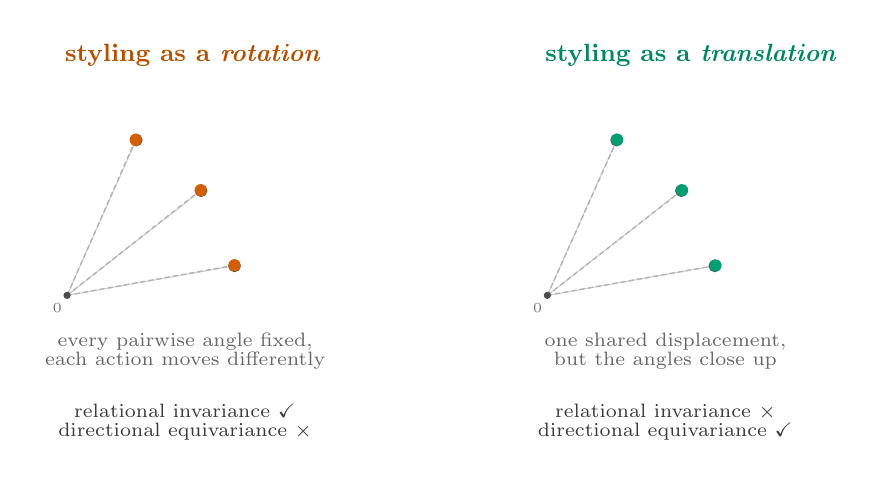
\begin{tikzpicture}[font=\small,line cap=round,line join=round,x=1cm,y=1cm]
\useasboundingbox (-0.5,-2.05) rectangle (10.05,3.4);
\begin{scope}[shift={(0.0,0)}]
\node[font=\small\bfseries,text=okverm!85!black,anchor=west] at (-0.15,3.05) {styling as a \emph{rotation}};
\draw[black!18,line width=0.4pt] (0,0) -- (2.127,0.375);
\draw[black!30,line width=0.5pt,dash pattern=on 1.6pt off 1.4pt] (0,0) -- (2.126,0.383);
\node[circle,draw=black!65,fill=white,inner sep=0pt,minimum size=4pt,line width=0.6pt] at (2.127,0.375) {};
\node[circle,fill=okverm,inner sep=0pt,minimum size=4.4pt] at (2.126,0.383) {};
\draw[black!18,line width=0.4pt] (0,0) -- (1.702,1.330);
\draw[black!30,line width=0.5pt,dash pattern=on 1.6pt off 1.4pt] (0,0) -- (1.697,1.336);
\node[circle,draw=black!65,fill=white,inner sep=0pt,minimum size=4pt,line width=0.6pt] at (1.702,1.330) {};
\node[circle,fill=okverm,inner sep=0pt,minimum size=4.4pt] at (1.697,1.336) {};
\draw[black!18,line width=0.4pt] (0,0) -- (0.879,1.973);
\draw[black!30,line width=0.5pt,dash pattern=on 1.6pt off 1.4pt] (0,0) -- (0.871,1.977);
\node[circle,draw=black!65,fill=white,inner sep=0pt,minimum size=4pt,line width=0.6pt] at (0.879,1.973) {};
\node[circle,fill=okverm,inner sep=0pt,minimum size=4.4pt] at (0.871,1.977) {};
\fill[black!70] (0,0) circle (1.3pt);
\node[font=\tiny,text=black!55,anchor=north east] at (0.06,0.02) {$0$};
\node[font=\scriptsize,text=black!60,align=center,anchor=north] at (1.5,-0.35) {every pairwise angle fixed,\\[-1pt] each action moves differently};
\node[font=\scriptsize,text=black!78,align=center,anchor=north] at (1.5,-1.25) {relational invariance \checkmark\\[-1pt] directional equivariance $\times$};
\end{scope}
\begin{scope}[shift={(6.1,0)}]
\node[font=\small\bfseries,text=okgreen!85!black,anchor=west] at (-0.15,3.05) {styling as a \emph{translation}};
\draw[black!18,line width=0.4pt] (0,0) -- (2.127,0.375);
\draw[black!30,line width=0.5pt,dash pattern=on 1.6pt off 1.4pt] (0,0) -- (2.136,0.380);
\node[circle,draw=black!65,fill=white,inner sep=0pt,minimum size=4pt,line width=0.6pt] at (2.127,0.375) {};
\node[circle,fill=okgreen,inner sep=0pt,minimum size=4.4pt] at (2.136,0.380) {};
\draw[black!18,line width=0.4pt] (0,0) -- (1.702,1.330);
\draw[black!30,line width=0.5pt,dash pattern=on 1.6pt off 1.4pt] (0,0) -- (1.711,1.335);
\node[circle,draw=black!65,fill=white,inner sep=0pt,minimum size=4pt,line width=0.6pt] at (1.702,1.330) {};
\node[circle,fill=okgreen,inner sep=0pt,minimum size=4.4pt] at (1.711,1.335) {};
\draw[black!18,line width=0.4pt] (0,0) -- (0.879,1.973);
\draw[black!30,line width=0.5pt,dash pattern=on 1.6pt off 1.4pt] (0,0) -- (0.887,1.978);
\node[circle,draw=black!65,fill=white,inner sep=0pt,minimum size=4pt,line width=0.6pt] at (0.879,1.973) {};
\node[circle,fill=okgreen,inner sep=0pt,minimum size=4.4pt] at (0.887,1.978) {};
\fill[black!70] (0,0) circle (1.3pt);
\node[font=\tiny,text=black!55,anchor=north east] at (0.06,0.02) {$0$};
\node[font=\scriptsize,text=black!60,align=center,anchor=north] at (1.5,-0.35) {one shared displacement,\\[-1pt] but the angles close up};
\node[font=\scriptsize,text=black!78,align=center,anchor=north] at (1.5,-1.25) {relational invariance $\times$\\[-1pt] directional equivariance \checkmark};
\end{scope}
\end{tikzpicture}
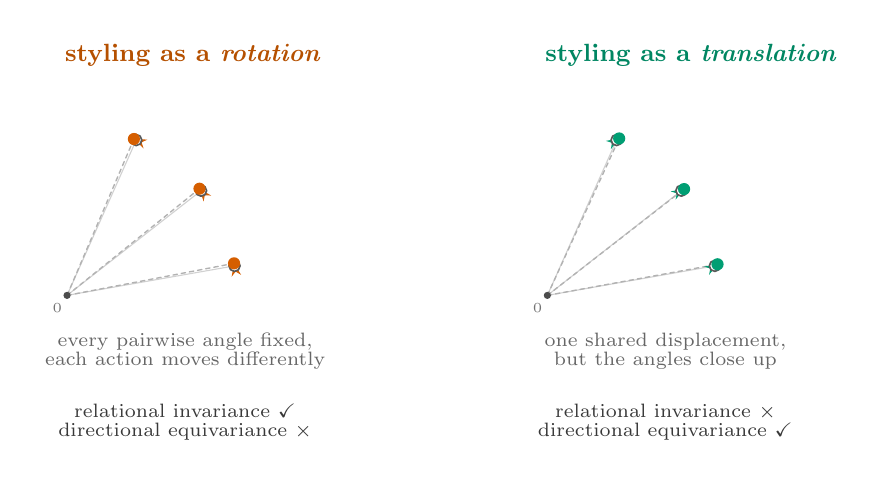
\begin{tikzpicture}[font=\small,line cap=round,line join=round,x=1cm,y=1cm]
\useasboundingbox (-0.5,-2.05) rectangle (10.05,3.4);
\begin{scope}[shift={(0.0,0)}]
\node[font=\small\bfseries,text=okverm!85!black,anchor=west] at (-0.15,3.05) {styling as a \emph{rotation}};
\draw[black!18,line width=0.4pt] (0,0) -- (2.127,0.375);
\draw[black!30,line width=0.5pt,dash pattern=on 1.6pt off 1.4pt] (0,0) -- (2.121,0.407);
\draw[-{Stealth[length=4.5pt,width=3.4pt]},okverm,line width=1.0pt] (2.127,0.375) -- (2.121,0.407);
\node[circle,draw=black!65,fill=white,inner sep=0pt,minimum size=4pt,line width=0.6pt] at (2.127,0.375) {};
\node[circle,fill=okverm,inner sep=0pt,minimum size=4.4pt] at (2.121,0.407) {};
\draw[black!18,line width=0.4pt] (0,0) -- (1.702,1.330);
\draw[black!30,line width=0.5pt,dash pattern=on 1.6pt off 1.4pt] (0,0) -- (1.682,1.355);
\draw[-{Stealth[length=4.5pt,width=3.4pt]},okverm,line width=1.0pt] (1.702,1.330) -- (1.682,1.355);
\node[circle,draw=black!65,fill=white,inner sep=0pt,minimum size=4pt,line width=0.6pt] at (1.702,1.330) {};
\node[circle,fill=okverm,inner sep=0pt,minimum size=4.4pt] at (1.682,1.355) {};
\draw[black!18,line width=0.4pt] (0,0) -- (0.879,1.973);
\draw[black!30,line width=0.5pt,dash pattern=on 1.6pt off 1.4pt] (0,0) -- (0.849,1.986);
\draw[-{Stealth[length=4.5pt,width=3.4pt]},okverm,line width=1.0pt] (0.879,1.973) -- (0.849,1.986);
\node[circle,draw=black!65,fill=white,inner sep=0pt,minimum size=4pt,line width=0.6pt] at (0.879,1.973) {};
\node[circle,fill=okverm,inner sep=0pt,minimum size=4.4pt] at (0.849,1.986) {};
\fill[black!70] (0,0) circle (1.3pt);
\node[font=\tiny,text=black!55,anchor=north east] at (0.06,0.02) {$0$};
\node[font=\scriptsize,text=black!60,align=center,anchor=north] at (1.5,-0.35) {every pairwise angle fixed,\\[-1pt] each action moves differently};
\node[font=\scriptsize,text=black!78,align=center,anchor=north] at (1.5,-1.25) {relational invariance \checkmark\\[-1pt] directional equivariance $\times$};
\end{scope}
\begin{scope}[shift={(6.1,0)}]
\node[font=\small\bfseries,text=okgreen!85!black,anchor=west] at (-0.15,3.05) {styling as a \emph{translation}};
\draw[black!18,line width=0.4pt] (0,0) -- (2.127,0.375);
\draw[black!30,line width=0.5pt,dash pattern=on 1.6pt off 1.4pt] (0,0) -- (2.161,0.395);
\draw[-{Stealth[length=4.5pt,width=3.4pt]},okgreen,line width=1.0pt] (2.127,0.375) -- (2.161,0.395);
\node[circle,draw=black!65,fill=white,inner sep=0pt,minimum size=4pt,line width=0.6pt] at (2.127,0.375) {};
\node[circle,fill=okgreen,inner sep=0pt,minimum size=4.4pt] at (2.161,0.395) {};
\draw[black!18,line width=0.4pt] (0,0) -- (1.702,1.330);
\draw[black!30,line width=0.5pt,dash pattern=on 1.6pt off 1.4pt] (0,0) -- (1.736,1.350);
\draw[-{Stealth[length=4.5pt,width=3.4pt]},okgreen,line width=1.0pt] (1.702,1.330) -- (1.736,1.350);
\node[circle,draw=black!65,fill=white,inner sep=0pt,minimum size=4pt,line width=0.6pt] at (1.702,1.330) {};
\node[circle,fill=okgreen,inner sep=0pt,minimum size=4.4pt] at (1.736,1.350) {};
\draw[black!18,line width=0.4pt] (0,0) -- (0.879,1.973);
\draw[black!30,line width=0.5pt,dash pattern=on 1.6pt off 1.4pt] (0,0) -- (0.912,1.993);
\draw[-{Stealth[length=4.5pt,width=3.4pt]},okgreen,line width=1.0pt] (0.879,1.973) -- (0.912,1.993);
\node[circle,draw=black!65,fill=white,inner sep=0pt,minimum size=4pt,line width=0.6pt] at (0.879,1.973) {};
\node[circle,fill=okgreen,inner sep=0pt,minimum size=4.4pt] at (0.912,1.993) {};
\fill[black!70] (0,0) circle (1.3pt);
\node[font=\tiny,text=black!55,anchor=north east] at (0.06,0.02) {$0$};
\node[font=\scriptsize,text=black!60,align=center,anchor=north] at (1.5,-0.35) {one shared displacement,\\[-1pt] but the angles close up};
\node[font=\scriptsize,text=black!78,align=center,anchor=north] at (1.5,-1.25) {relational invariance $\times$\\[-1pt] directional equivariance \checkmark};
\end{scope}
\end{tikzpicture}
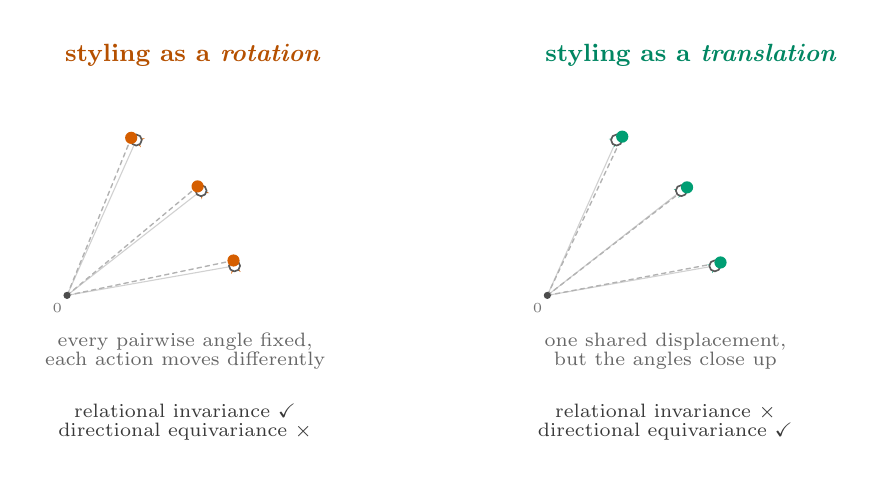
\begin{tikzpicture}[font=\small,line cap=round,line join=round,x=1cm,y=1cm]
\useasboundingbox (-0.5,-2.05) rectangle (10.05,3.4);
\begin{scope}[shift={(0.0,0)}]
\node[font=\small\bfseries,text=okverm!85!black,anchor=west] at (-0.15,3.05) {styling as a \emph{rotation}};
\draw[black!18,line width=0.4pt] (0,0) -- (2.127,0.375);
\draw[black!30,line width=0.5pt,dash pattern=on 1.6pt off 1.4pt] (0,0) -- (2.114,0.443);
\draw[-{Stealth[length=4.5pt,width=3.4pt]},okverm,line width=1.0pt] (2.127,0.375) -- (2.114,0.443);
\node[circle,draw=black!65,fill=white,inner sep=0pt,minimum size=4pt,line width=0.6pt] at (2.127,0.375) {};
\node[circle,fill=okverm,inner sep=0pt,minimum size=4.4pt] at (2.114,0.443) {};
\draw[black!18,line width=0.4pt] (0,0) -- (1.702,1.330);
\draw[black!30,line width=0.5pt,dash pattern=on 1.6pt off 1.4pt] (0,0) -- (1.658,1.384);
\draw[-{Stealth[length=4.5pt,width=3.4pt]},okverm,line width=1.0pt] (1.702,1.330) -- (1.658,1.384);
\node[circle,draw=black!65,fill=white,inner sep=0pt,minimum size=4pt,line width=0.6pt] at (1.702,1.330) {};
\node[circle,fill=okverm,inner sep=0pt,minimum size=4.4pt] at (1.658,1.384) {};
\draw[black!18,line width=0.4pt] (0,0) -- (0.879,1.973);
\draw[black!30,line width=0.5pt,dash pattern=on 1.6pt off 1.4pt] (0,0) -- (0.815,2.001);
\draw[-{Stealth[length=4.5pt,width=3.4pt]},okverm,line width=1.0pt] (0.879,1.973) -- (0.815,2.001);
\node[circle,draw=black!65,fill=white,inner sep=0pt,minimum size=4pt,line width=0.6pt] at (0.879,1.973) {};
\node[circle,fill=okverm,inner sep=0pt,minimum size=4.4pt] at (0.815,2.001) {};
\fill[black!70] (0,0) circle (1.3pt);
\node[font=\tiny,text=black!55,anchor=north east] at (0.06,0.02) {$0$};
\node[font=\scriptsize,text=black!60,align=center,anchor=north] at (1.5,-0.35) {every pairwise angle fixed,\\[-1pt] each action moves differently};
\node[font=\scriptsize,text=black!78,align=center,anchor=north] at (1.5,-1.25) {relational invariance \checkmark\\[-1pt] directional equivariance $\times$};
\end{scope}
\begin{scope}[shift={(6.1,0)}]
\node[font=\small\bfseries,text=okgreen!85!black,anchor=west] at (-0.15,3.05) {styling as a \emph{translation}};
\draw[black!18,line width=0.4pt] (0,0) -- (2.127,0.375);
\draw[black!30,line width=0.5pt,dash pattern=on 1.6pt off 1.4pt] (0,0) -- (2.199,0.418);
\draw[-{Stealth[length=4.5pt,width=3.4pt]},okgreen,line width=1.0pt] (2.127,0.375) -- (2.199,0.418);
\node[circle,draw=black!65,fill=white,inner sep=0pt,minimum size=4pt,line width=0.6pt] at (2.127,0.375) {};
\node[circle,fill=okgreen,inner sep=0pt,minimum size=4.4pt] at (2.199,0.418) {};
\draw[black!18,line width=0.4pt] (0,0) -- (1.702,1.330);
\draw[black!30,line width=0.5pt,dash pattern=on 1.6pt off 1.4pt] (0,0) -- (1.774,1.372);
\draw[-{Stealth[length=4.5pt,width=3.4pt]},okgreen,line width=1.0pt] (1.702,1.330) -- (1.774,1.372);
\node[circle,draw=black!65,fill=white,inner sep=0pt,minimum size=4pt,line width=0.6pt] at (1.702,1.330) {};
\node[circle,fill=okgreen,inner sep=0pt,minimum size=4.4pt] at (1.774,1.372) {};
\draw[black!18,line width=0.4pt] (0,0) -- (0.879,1.973);
\draw[black!30,line width=0.5pt,dash pattern=on 1.6pt off 1.4pt] (0,0) -- (0.951,2.016);
\draw[-{Stealth[length=4.5pt,width=3.4pt]},okgreen,line width=1.0pt] (0.879,1.973) -- (0.951,2.016);
\node[circle,draw=black!65,fill=white,inner sep=0pt,minimum size=4pt,line width=0.6pt] at (0.879,1.973) {};
\node[circle,fill=okgreen,inner sep=0pt,minimum size=4.4pt] at (0.951,2.016) {};
\fill[black!70] (0,0) circle (1.3pt);
\node[font=\tiny,text=black!55,anchor=north east] at (0.06,0.02) {$0$};
\node[font=\scriptsize,text=black!60,align=center,anchor=north] at (1.5,-0.35) {one shared displacement,\\[-1pt] but the angles close up};
\node[font=\scriptsize,text=black!78,align=center,anchor=north] at (1.5,-1.25) {relational invariance $\times$\\[-1pt] directional equivariance \checkmark};
\end{scope}
\end{tikzpicture}
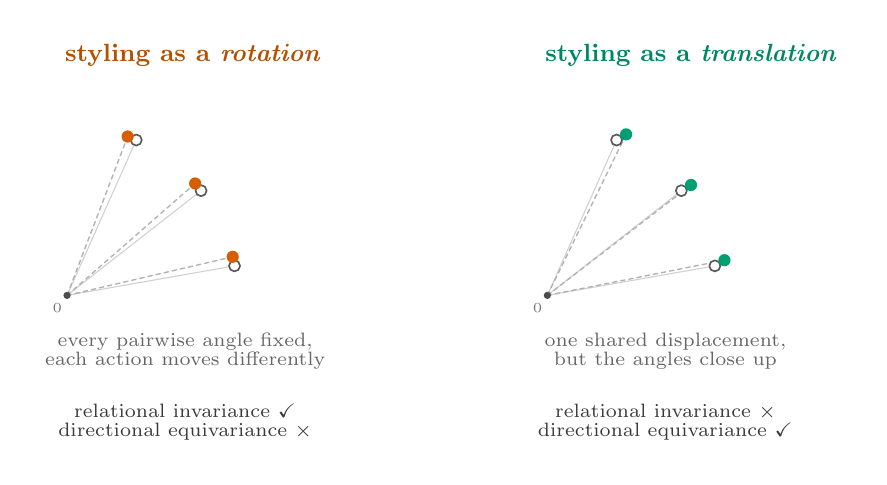
\begin{tikzpicture}[font=\small,line cap=round,line join=round,x=1cm,y=1cm]
\useasboundingbox (-0.5,-2.05) rectangle (10.05,3.4);
\begin{scope}[shift={(0.0,0)}]
\node[font=\small\bfseries,text=okverm!85!black,anchor=west] at (-0.15,3.05) {styling as a \emph{rotation}};
\draw[black!18,line width=0.4pt] (0,0) -- (2.127,0.375);
\draw[black!30,line width=0.5pt,dash pattern=on 1.6pt off 1.4pt] (0,0) -- (2.104,0.490);
\draw[-{Stealth[length=4.5pt,width=3.4pt]},okverm,line width=1.0pt] (2.127,0.375) -- (2.104,0.490);
\node[circle,draw=black!65,fill=white,inner sep=0pt,minimum size=4pt,line width=0.6pt] at (2.127,0.375) {};
\node[circle,fill=okverm,inner sep=0pt,minimum size=4.4pt] at (2.104,0.490) {};
\draw[black!18,line width=0.4pt] (0,0) -- (1.702,1.330);
\draw[black!30,line width=0.5pt,dash pattern=on 1.6pt off 1.4pt] (0,0) -- (1.627,1.421);
\draw[-{Stealth[length=4.5pt,width=3.4pt]},okverm,line width=1.0pt] (1.702,1.330) -- (1.627,1.421);
\node[circle,draw=black!65,fill=white,inner sep=0pt,minimum size=4pt,line width=0.6pt] at (1.702,1.330) {};
\node[circle,fill=okverm,inner sep=0pt,minimum size=4.4pt] at (1.627,1.421) {};
\draw[black!18,line width=0.4pt] (0,0) -- (0.879,1.973);
\draw[black!30,line width=0.5pt,dash pattern=on 1.6pt off 1.4pt] (0,0) -- (0.770,2.018);
\draw[-{Stealth[length=4.5pt,width=3.4pt]},okverm,line width=1.0pt] (0.879,1.973) -- (0.770,2.018);
\node[circle,draw=black!65,fill=white,inner sep=0pt,minimum size=4pt,line width=0.6pt] at (0.879,1.973) {};
\node[circle,fill=okverm,inner sep=0pt,minimum size=4.4pt] at (0.770,2.018) {};
\fill[black!70] (0,0) circle (1.3pt);
\node[font=\tiny,text=black!55,anchor=north east] at (0.06,0.02) {$0$};
\node[font=\scriptsize,text=black!60,align=center,anchor=north] at (1.5,-0.35) {every pairwise angle fixed,\\[-1pt] each action moves differently};
\node[font=\scriptsize,text=black!78,align=center,anchor=north] at (1.5,-1.25) {relational invariance \checkmark\\[-1pt] directional equivariance $\times$};
\end{scope}
\begin{scope}[shift={(6.1,0)}]
\node[font=\small\bfseries,text=okgreen!85!black,anchor=west] at (-0.15,3.05) {styling as a \emph{translation}};
\draw[black!18,line width=0.4pt] (0,0) -- (2.127,0.375);
\draw[black!30,line width=0.5pt,dash pattern=on 1.6pt off 1.4pt] (0,0) -- (2.249,0.447);
\draw[-{Stealth[length=4.5pt,width=3.4pt]},okgreen,line width=1.0pt] (2.127,0.375) -- (2.249,0.447);
\node[circle,draw=black!65,fill=white,inner sep=0pt,minimum size=4pt,line width=0.6pt] at (2.127,0.375) {};
\node[circle,fill=okgreen,inner sep=0pt,minimum size=4.4pt] at (2.249,0.447) {};
\draw[black!18,line width=0.4pt] (0,0) -- (1.702,1.330);
\draw[black!30,line width=0.5pt,dash pattern=on 1.6pt off 1.4pt] (0,0) -- (1.824,1.402);
\draw[-{Stealth[length=4.5pt,width=3.4pt]},okgreen,line width=1.0pt] (1.702,1.330) -- (1.824,1.402);
\node[circle,draw=black!65,fill=white,inner sep=0pt,minimum size=4pt,line width=0.6pt] at (1.702,1.330) {};
\node[circle,fill=okgreen,inner sep=0pt,minimum size=4.4pt] at (1.824,1.402) {};
\draw[black!18,line width=0.4pt] (0,0) -- (0.879,1.973);
\draw[black!30,line width=0.5pt,dash pattern=on 1.6pt off 1.4pt] (0,0) -- (1.000,2.045);
\draw[-{Stealth[length=4.5pt,width=3.4pt]},okgreen,line width=1.0pt] (0.879,1.973) -- (1.000,2.045);
\node[circle,draw=black!65,fill=white,inner sep=0pt,minimum size=4pt,line width=0.6pt] at (0.879,1.973) {};
\node[circle,fill=okgreen,inner sep=0pt,minimum size=4.4pt] at (1.000,2.045) {};
\fill[black!70] (0,0) circle (1.3pt);
\node[font=\tiny,text=black!55,anchor=north east] at (0.06,0.02) {$0$};
\node[font=\scriptsize,text=black!60,align=center,anchor=north] at (1.5,-0.35) {one shared displacement,\\[-1pt] but the angles close up};
\node[font=\scriptsize,text=black!78,align=center,anchor=north] at (1.5,-1.25) {relational invariance $\times$\\[-1pt] directional equivariance \checkmark};
\end{scope}
\end{tikzpicture}
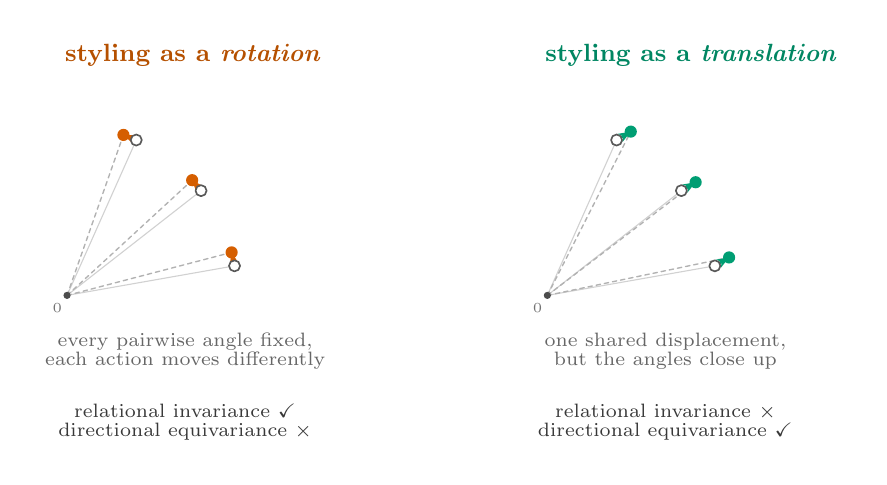
\begin{tikzpicture}[font=\small,line cap=round,line join=round,x=1cm,y=1cm]
\useasboundingbox (-0.5,-2.05) rectangle (10.05,3.4);
\begin{scope}[shift={(0.0,0)}]
\node[font=\small\bfseries,text=okverm!85!black,anchor=west] at (-0.15,3.05) {styling as a \emph{rotation}};
\draw[black!18,line width=0.4pt] (0,0) -- (2.127,0.375);
\draw[black!30,line width=0.5pt,dash pattern=on 1.6pt off 1.4pt] (0,0) -- (2.090,0.546);
\draw[-{Stealth[length=4.5pt,width=3.4pt]},okverm,line width=1.0pt] (2.127,0.375) -- (2.090,0.546);
\node[circle,draw=black!65,fill=white,inner sep=0pt,minimum size=4pt,line width=0.6pt] at (2.127,0.375) {};
\node[circle,fill=okverm,inner sep=0pt,minimum size=4.4pt] at (2.090,0.546) {};
\draw[black!18,line width=0.4pt] (0,0) -- (1.702,1.330);
\draw[black!30,line width=0.5pt,dash pattern=on 1.6pt off 1.4pt] (0,0) -- (1.589,1.463);
\draw[-{Stealth[length=4.5pt,width=3.4pt]},okverm,line width=1.0pt] (1.702,1.330) -- (1.589,1.463);
\node[circle,draw=black!65,fill=white,inner sep=0pt,minimum size=4pt,line width=0.6pt] at (1.702,1.330) {};
\node[circle,fill=okverm,inner sep=0pt,minimum size=4.4pt] at (1.589,1.463) {};
\draw[black!18,line width=0.4pt] (0,0) -- (0.879,1.973);
\draw[black!30,line width=0.5pt,dash pattern=on 1.6pt off 1.4pt] (0,0) -- (0.716,2.038);
\draw[-{Stealth[length=4.5pt,width=3.4pt]},okverm,line width=1.0pt] (0.879,1.973) -- (0.716,2.038);
\node[circle,draw=black!65,fill=white,inner sep=0pt,minimum size=4pt,line width=0.6pt] at (0.879,1.973) {};
\node[circle,fill=okverm,inner sep=0pt,minimum size=4.4pt] at (0.716,2.038) {};
\fill[black!70] (0,0) circle (1.3pt);
\node[font=\tiny,text=black!55,anchor=north east] at (0.06,0.02) {$0$};
\node[font=\scriptsize,text=black!60,align=center,anchor=north] at (1.5,-0.35) {every pairwise angle fixed,\\[-1pt] each action moves differently};
\node[font=\scriptsize,text=black!78,align=center,anchor=north] at (1.5,-1.25) {relational invariance \checkmark\\[-1pt] directional equivariance $\times$};
\end{scope}
\begin{scope}[shift={(6.1,0)}]
\node[font=\small\bfseries,text=okgreen!85!black,anchor=west] at (-0.15,3.05) {styling as a \emph{translation}};
\draw[black!18,line width=0.4pt] (0,0) -- (2.127,0.375);
\draw[black!30,line width=0.5pt,dash pattern=on 1.6pt off 1.4pt] (0,0) -- (2.308,0.482);
\draw[-{Stealth[length=4.5pt,width=3.4pt]},okgreen,line width=1.0pt] (2.127,0.375) -- (2.308,0.482);
\node[circle,draw=black!65,fill=white,inner sep=0pt,minimum size=4pt,line width=0.6pt] at (2.127,0.375) {};
\node[circle,fill=okgreen,inner sep=0pt,minimum size=4.4pt] at (2.308,0.482) {};
\draw[black!18,line width=0.4pt] (0,0) -- (1.702,1.330);
\draw[black!30,line width=0.5pt,dash pattern=on 1.6pt off 1.4pt] (0,0) -- (1.883,1.437);
\draw[-{Stealth[length=4.5pt,width=3.4pt]},okgreen,line width=1.0pt] (1.702,1.330) -- (1.883,1.437);
\node[circle,draw=black!65,fill=white,inner sep=0pt,minimum size=4pt,line width=0.6pt] at (1.702,1.330) {};
\node[circle,fill=okgreen,inner sep=0pt,minimum size=4.4pt] at (1.883,1.437) {};
\draw[black!18,line width=0.4pt] (0,0) -- (0.879,1.973);
\draw[black!30,line width=0.5pt,dash pattern=on 1.6pt off 1.4pt] (0,0) -- (1.059,2.080);
\draw[-{Stealth[length=4.5pt,width=3.4pt]},okgreen,line width=1.0pt] (0.879,1.973) -- (1.059,2.080);
\node[circle,draw=black!65,fill=white,inner sep=0pt,minimum size=4pt,line width=0.6pt] at (0.879,1.973) {};
\node[circle,fill=okgreen,inner sep=0pt,minimum size=4.4pt] at (1.059,2.080) {};
\fill[black!70] (0,0) circle (1.3pt);
\node[font=\tiny,text=black!55,anchor=north east] at (0.06,0.02) {$0$};
\node[font=\scriptsize,text=black!60,align=center,anchor=north] at (1.5,-0.35) {one shared displacement,\\[-1pt] but the angles close up};
\node[font=\scriptsize,text=black!78,align=center,anchor=north] at (1.5,-1.25) {relational invariance $\times$\\[-1pt] directional equivariance \checkmark};
\end{scope}
\end{tikzpicture}
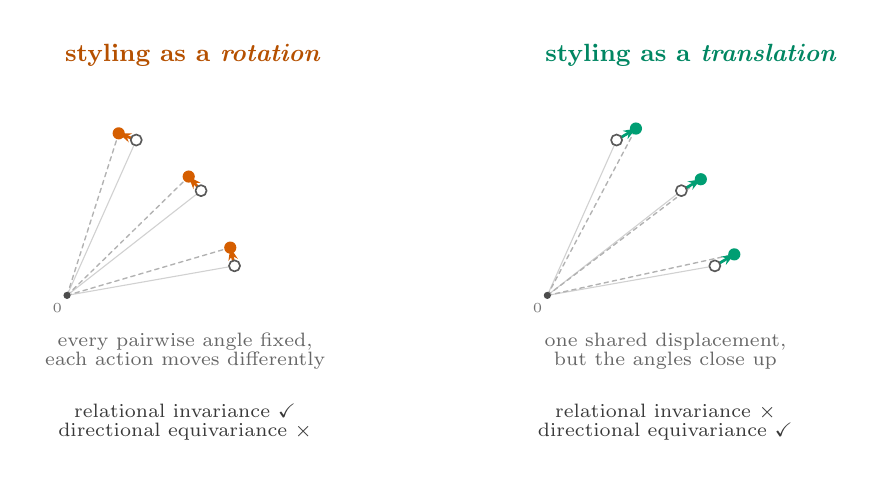
\begin{tikzpicture}[font=\small,line cap=round,line join=round,x=1cm,y=1cm]
\useasboundingbox (-0.5,-2.05) rectangle (10.05,3.4);
\begin{scope}[shift={(0.0,0)}]
\node[font=\small\bfseries,text=okverm!85!black,anchor=west] at (-0.15,3.05) {styling as a \emph{rotation}};
\draw[black!18,line width=0.4pt] (0,0) -- (2.127,0.375);
\draw[black!30,line width=0.5pt,dash pattern=on 1.6pt off 1.4pt] (0,0) -- (2.073,0.607);
\draw[-{Stealth[length=4.5pt,width=3.4pt]},okverm,line width=1.0pt] (2.127,0.375) -- (2.073,0.607);
\node[circle,draw=black!65,fill=white,inner sep=0pt,minimum size=4pt,line width=0.6pt] at (2.127,0.375) {};
\node[circle,fill=okverm,inner sep=0pt,minimum size=4.4pt] at (2.073,0.607) {};
\draw[black!18,line width=0.4pt] (0,0) -- (1.702,1.330);
\draw[black!30,line width=0.5pt,dash pattern=on 1.6pt off 1.4pt] (0,0) -- (1.545,1.509);
\draw[-{Stealth[length=4.5pt,width=3.4pt]},okverm,line width=1.0pt] (1.702,1.330) -- (1.545,1.509);
\node[circle,draw=black!65,fill=white,inner sep=0pt,minimum size=4pt,line width=0.6pt] at (1.702,1.330) {};
\node[circle,fill=okverm,inner sep=0pt,minimum size=4.4pt] at (1.545,1.509) {};
\draw[black!18,line width=0.4pt] (0,0) -- (0.879,1.973);
\draw[black!30,line width=0.5pt,dash pattern=on 1.6pt off 1.4pt] (0,0) -- (0.656,2.058);
\draw[-{Stealth[length=4.5pt,width=3.4pt]},okverm,line width=1.0pt] (0.879,1.973) -- (0.656,2.058);
\node[circle,draw=black!65,fill=white,inner sep=0pt,minimum size=4pt,line width=0.6pt] at (0.879,1.973) {};
\node[circle,fill=okverm,inner sep=0pt,minimum size=4.4pt] at (0.656,2.058) {};
\fill[black!70] (0,0) circle (1.3pt);
\node[font=\tiny,text=black!55,anchor=north east] at (0.06,0.02) {$0$};
\node[font=\scriptsize,text=black!60,align=center,anchor=north] at (1.5,-0.35) {every pairwise angle fixed,\\[-1pt] each action moves differently};
\node[font=\scriptsize,text=black!78,align=center,anchor=north] at (1.5,-1.25) {relational invariance \checkmark\\[-1pt] directional equivariance $\times$};
\end{scope}
\begin{scope}[shift={(6.1,0)}]
\node[font=\small\bfseries,text=okgreen!85!black,anchor=west] at (-0.15,3.05) {styling as a \emph{translation}};
\draw[black!18,line width=0.4pt] (0,0) -- (2.127,0.375);
\draw[black!30,line width=0.5pt,dash pattern=on 1.6pt off 1.4pt] (0,0) -- (2.374,0.521);
\draw[-{Stealth[length=4.5pt,width=3.4pt]},okgreen,line width=1.0pt] (2.127,0.375) -- (2.374,0.521);
\node[circle,draw=black!65,fill=white,inner sep=0pt,minimum size=4pt,line width=0.6pt] at (2.127,0.375) {};
\node[circle,fill=okgreen,inner sep=0pt,minimum size=4.4pt] at (2.374,0.521) {};
\draw[black!18,line width=0.4pt] (0,0) -- (1.702,1.330);
\draw[black!30,line width=0.5pt,dash pattern=on 1.6pt off 1.4pt] (0,0) -- (1.949,1.475);
\draw[-{Stealth[length=4.5pt,width=3.4pt]},okgreen,line width=1.0pt] (1.702,1.330) -- (1.949,1.475);
\node[circle,draw=black!65,fill=white,inner sep=0pt,minimum size=4pt,line width=0.6pt] at (1.702,1.330) {};
\node[circle,fill=okgreen,inner sep=0pt,minimum size=4.4pt] at (1.949,1.475) {};
\draw[black!18,line width=0.4pt] (0,0) -- (0.879,1.973);
\draw[black!30,line width=0.5pt,dash pattern=on 1.6pt off 1.4pt] (0,0) -- (1.125,2.119);
\draw[-{Stealth[length=4.5pt,width=3.4pt]},okgreen,line width=1.0pt] (0.879,1.973) -- (1.125,2.119);
\node[circle,draw=black!65,fill=white,inner sep=0pt,minimum size=4pt,line width=0.6pt] at (0.879,1.973) {};
\node[circle,fill=okgreen,inner sep=0pt,minimum size=4.4pt] at (1.125,2.119) {};
\fill[black!70] (0,0) circle (1.3pt);
\node[font=\tiny,text=black!55,anchor=north east] at (0.06,0.02) {$0$};
\node[font=\scriptsize,text=black!60,align=center,anchor=north] at (1.5,-0.35) {one shared displacement,\\[-1pt] but the angles close up};
\node[font=\scriptsize,text=black!78,align=center,anchor=north] at (1.5,-1.25) {relational invariance $\times$\\[-1pt] directional equivariance \checkmark};
\end{scope}
\end{tikzpicture}
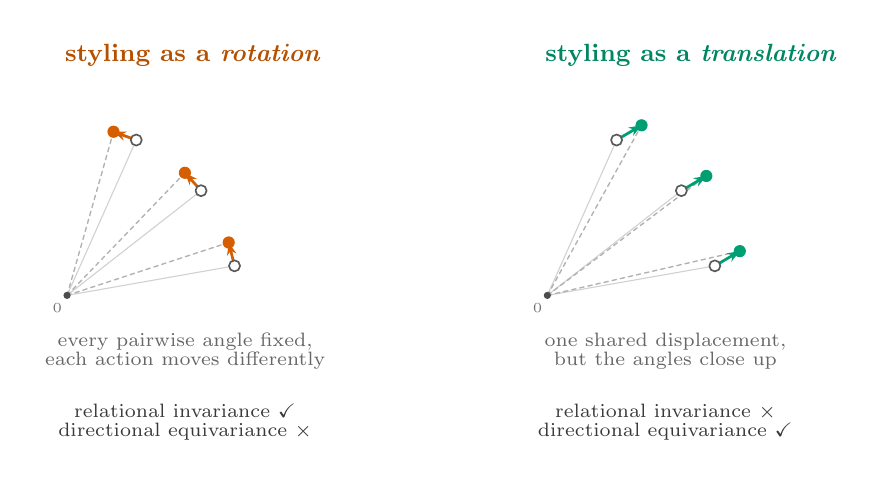
\begin{tikzpicture}[font=\small,line cap=round,line join=round,x=1cm,y=1cm]
\useasboundingbox (-0.5,-2.05) rectangle (10.05,3.4);
\begin{scope}[shift={(0.0,0)}]
\node[font=\small\bfseries,text=okverm!85!black,anchor=west] at (-0.15,3.05) {styling as a \emph{rotation}};
\draw[black!18,line width=0.4pt] (0,0) -- (2.127,0.375);
\draw[black!30,line width=0.5pt,dash pattern=on 1.6pt off 1.4pt] (0,0) -- (2.053,0.672);
\draw[-{Stealth[length=4.5pt,width=3.4pt]},okverm,line width=1.0pt] (2.127,0.375) -- (2.053,0.672);
\node[circle,draw=black!65,fill=white,inner sep=0pt,minimum size=4pt,line width=0.6pt] at (2.127,0.375) {};
\node[circle,fill=okverm,inner sep=0pt,minimum size=4.4pt] at (2.053,0.672) {};
\draw[black!18,line width=0.4pt] (0,0) -- (1.702,1.330);
\draw[black!30,line width=0.5pt,dash pattern=on 1.6pt off 1.4pt] (0,0) -- (1.497,1.557);
\draw[-{Stealth[length=4.5pt,width=3.4pt]},okverm,line width=1.0pt] (1.702,1.330) -- (1.497,1.557);
\node[circle,draw=black!65,fill=white,inner sep=0pt,minimum size=4pt,line width=0.6pt] at (1.702,1.330) {};
\node[circle,fill=okverm,inner sep=0pt,minimum size=4.4pt] at (1.497,1.557) {};
\draw[black!18,line width=0.4pt] (0,0) -- (0.879,1.973);
\draw[black!30,line width=0.5pt,dash pattern=on 1.6pt off 1.4pt] (0,0) -- (0.590,2.078);
\draw[-{Stealth[length=4.5pt,width=3.4pt]},okverm,line width=1.0pt] (0.879,1.973) -- (0.590,2.078);
\node[circle,draw=black!65,fill=white,inner sep=0pt,minimum size=4pt,line width=0.6pt] at (0.879,1.973) {};
\node[circle,fill=okverm,inner sep=0pt,minimum size=4.4pt] at (0.590,2.078) {};
\fill[black!70] (0,0) circle (1.3pt);
\node[font=\tiny,text=black!55,anchor=north east] at (0.06,0.02) {$0$};
\node[font=\scriptsize,text=black!60,align=center,anchor=north] at (1.5,-0.35) {every pairwise angle fixed,\\[-1pt] each action moves differently};
\node[font=\scriptsize,text=black!78,align=center,anchor=north] at (1.5,-1.25) {relational invariance \checkmark\\[-1pt] directional equivariance $\times$};
\end{scope}
\begin{scope}[shift={(6.1,0)}]
\node[font=\small\bfseries,text=okgreen!85!black,anchor=west] at (-0.15,3.05) {styling as a \emph{translation}};
\draw[black!18,line width=0.4pt] (0,0) -- (2.127,0.375);
\draw[black!30,line width=0.5pt,dash pattern=on 1.6pt off 1.4pt] (0,0) -- (2.444,0.562);
\draw[-{Stealth[length=4.5pt,width=3.4pt]},okgreen,line width=1.0pt] (2.127,0.375) -- (2.444,0.562);
\node[circle,draw=black!65,fill=white,inner sep=0pt,minimum size=4pt,line width=0.6pt] at (2.127,0.375) {};
\node[circle,fill=okgreen,inner sep=0pt,minimum size=4.4pt] at (2.444,0.562) {};
\draw[black!18,line width=0.4pt] (0,0) -- (1.702,1.330);
\draw[black!30,line width=0.5pt,dash pattern=on 1.6pt off 1.4pt] (0,0) -- (2.019,1.517);
\draw[-{Stealth[length=4.5pt,width=3.4pt]},okgreen,line width=1.0pt] (1.702,1.330) -- (2.019,1.517);
\node[circle,draw=black!65,fill=white,inner sep=0pt,minimum size=4pt,line width=0.6pt] at (1.702,1.330) {};
\node[circle,fill=okgreen,inner sep=0pt,minimum size=4.4pt] at (2.019,1.517) {};
\draw[black!18,line width=0.4pt] (0,0) -- (0.879,1.973);
\draw[black!30,line width=0.5pt,dash pattern=on 1.6pt off 1.4pt] (0,0) -- (1.196,2.160);
\draw[-{Stealth[length=4.5pt,width=3.4pt]},okgreen,line width=1.0pt] (0.879,1.973) -- (1.196,2.160);
\node[circle,draw=black!65,fill=white,inner sep=0pt,minimum size=4pt,line width=0.6pt] at (0.879,1.973) {};
\node[circle,fill=okgreen,inner sep=0pt,minimum size=4.4pt] at (1.196,2.160) {};
\fill[black!70] (0,0) circle (1.3pt);
\node[font=\tiny,text=black!55,anchor=north east] at (0.06,0.02) {$0$};
\node[font=\scriptsize,text=black!60,align=center,anchor=north] at (1.5,-0.35) {one shared displacement,\\[-1pt] but the angles close up};
\node[font=\scriptsize,text=black!78,align=center,anchor=north] at (1.5,-1.25) {relational invariance $\times$\\[-1pt] directional equivariance \checkmark};
\end{scope}
\end{tikzpicture}
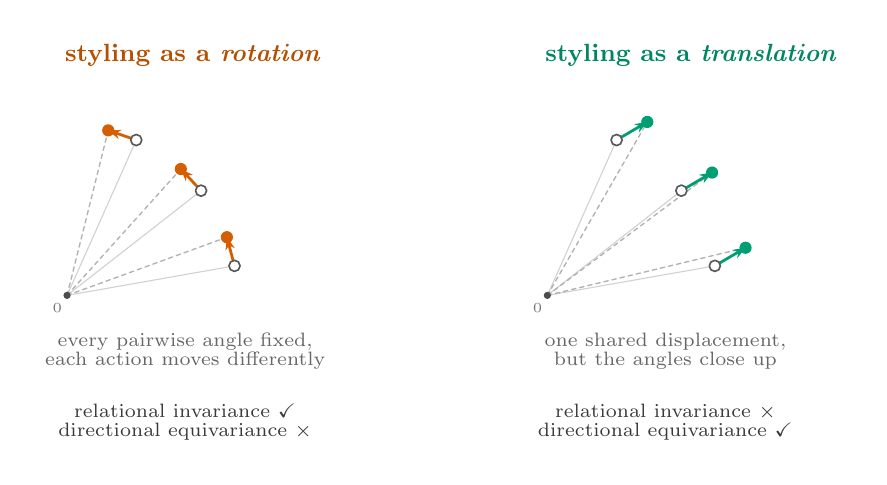
\begin{tikzpicture}[font=\small,line cap=round,line join=round,x=1cm,y=1cm]
\useasboundingbox (-0.5,-2.05) rectangle (10.05,3.4);
\begin{scope}[shift={(0.0,0)}]
\node[font=\small\bfseries,text=okverm!85!black,anchor=west] at (-0.15,3.05) {styling as a \emph{rotation}};
\draw[black!18,line width=0.4pt] (0,0) -- (2.127,0.375);
\draw[black!30,line width=0.5pt,dash pattern=on 1.6pt off 1.4pt] (0,0) -- (2.030,0.739);
\draw[-{Stealth[length=4.5pt,width=3.4pt]},okverm,line width=1.0pt] (2.127,0.375) -- (2.030,0.739);
\node[circle,draw=black!65,fill=white,inner sep=0pt,minimum size=4pt,line width=0.6pt] at (2.127,0.375) {};
\node[circle,fill=okverm,inner sep=0pt,minimum size=4.4pt] at (2.030,0.739) {};
\draw[black!18,line width=0.4pt] (0,0) -- (1.702,1.330);
\draw[black!30,line width=0.5pt,dash pattern=on 1.6pt off 1.4pt] (0,0) -- (1.445,1.605);
\draw[-{Stealth[length=4.5pt,width=3.4pt]},okverm,line width=1.0pt] (1.702,1.330) -- (1.445,1.605);
\node[circle,draw=black!65,fill=white,inner sep=0pt,minimum size=4pt,line width=0.6pt] at (1.702,1.330) {};
\node[circle,fill=okverm,inner sep=0pt,minimum size=4.4pt] at (1.445,1.605) {};
\draw[black!18,line width=0.4pt] (0,0) -- (0.879,1.973);
\draw[black!30,line width=0.5pt,dash pattern=on 1.6pt off 1.4pt] (0,0) -- (0.523,2.096);
\draw[-{Stealth[length=4.5pt,width=3.4pt]},okverm,line width=1.0pt] (0.879,1.973) -- (0.523,2.096);
\node[circle,draw=black!65,fill=white,inner sep=0pt,minimum size=4pt,line width=0.6pt] at (0.879,1.973) {};
\node[circle,fill=okverm,inner sep=0pt,minimum size=4.4pt] at (0.523,2.096) {};
\fill[black!70] (0,0) circle (1.3pt);
\node[font=\tiny,text=black!55,anchor=north east] at (0.06,0.02) {$0$};
\node[font=\scriptsize,text=black!60,align=center,anchor=north] at (1.5,-0.35) {every pairwise angle fixed,\\[-1pt] each action moves differently};
\node[font=\scriptsize,text=black!78,align=center,anchor=north] at (1.5,-1.25) {relational invariance \checkmark\\[-1pt] directional equivariance $\times$};
\end{scope}
\begin{scope}[shift={(6.1,0)}]
\node[font=\small\bfseries,text=okgreen!85!black,anchor=west] at (-0.15,3.05) {styling as a \emph{translation}};
\draw[black!18,line width=0.4pt] (0,0) -- (2.127,0.375);
\draw[black!30,line width=0.5pt,dash pattern=on 1.6pt off 1.4pt] (0,0) -- (2.517,0.605);
\draw[-{Stealth[length=4.5pt,width=3.4pt]},okgreen,line width=1.0pt] (2.127,0.375) -- (2.517,0.605);
\node[circle,draw=black!65,fill=white,inner sep=0pt,minimum size=4pt,line width=0.6pt] at (2.127,0.375) {};
\node[circle,fill=okgreen,inner sep=0pt,minimum size=4.4pt] at (2.517,0.605) {};
\draw[black!18,line width=0.4pt] (0,0) -- (1.702,1.330);
\draw[black!30,line width=0.5pt,dash pattern=on 1.6pt off 1.4pt] (0,0) -- (2.092,1.560);
\draw[-{Stealth[length=4.5pt,width=3.4pt]},okgreen,line width=1.0pt] (1.702,1.330) -- (2.092,1.560);
\node[circle,draw=black!65,fill=white,inner sep=0pt,minimum size=4pt,line width=0.6pt] at (1.702,1.330) {};
\node[circle,fill=okgreen,inner sep=0pt,minimum size=4.4pt] at (2.092,1.560) {};
\draw[black!18,line width=0.4pt] (0,0) -- (0.879,1.973);
\draw[black!30,line width=0.5pt,dash pattern=on 1.6pt off 1.4pt] (0,0) -- (1.269,2.203);
\draw[-{Stealth[length=4.5pt,width=3.4pt]},okgreen,line width=1.0pt] (0.879,1.973) -- (1.269,2.203);
\node[circle,draw=black!65,fill=white,inner sep=0pt,minimum size=4pt,line width=0.6pt] at (0.879,1.973) {};
\node[circle,fill=okgreen,inner sep=0pt,minimum size=4.4pt] at (1.269,2.203) {};
\fill[black!70] (0,0) circle (1.3pt);
\node[font=\tiny,text=black!55,anchor=north east] at (0.06,0.02) {$0$};
\node[font=\scriptsize,text=black!60,align=center,anchor=north] at (1.5,-0.35) {one shared displacement,\\[-1pt] but the angles close up};
\node[font=\scriptsize,text=black!78,align=center,anchor=north] at (1.5,-1.25) {relational invariance $\times$\\[-1pt] directional equivariance \checkmark};
\end{scope}
\end{tikzpicture}
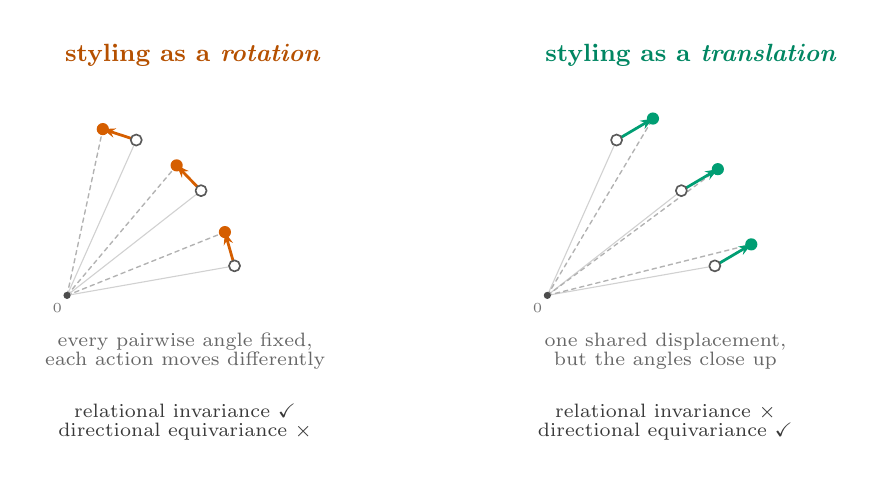
\begin{tikzpicture}[font=\small,line cap=round,line join=round,x=1cm,y=1cm]
\useasboundingbox (-0.5,-2.05) rectangle (10.05,3.4);
\begin{scope}[shift={(0.0,0)}]
\node[font=\small\bfseries,text=okverm!85!black,anchor=west] at (-0.15,3.05) {styling as a \emph{rotation}};
\draw[black!18,line width=0.4pt] (0,0) -- (2.127,0.375);
\draw[black!30,line width=0.5pt,dash pattern=on 1.6pt off 1.4pt] (0,0) -- (2.005,0.804);
\draw[-{Stealth[length=4.5pt,width=3.4pt]},okverm,line width=1.0pt] (2.127,0.375) -- (2.005,0.804);
\node[circle,draw=black!65,fill=white,inner sep=0pt,minimum size=4pt,line width=0.6pt] at (2.127,0.375) {};
\node[circle,fill=okverm,inner sep=0pt,minimum size=4.4pt] at (2.005,0.804) {};
\draw[black!18,line width=0.4pt] (0,0) -- (1.702,1.330);
\draw[black!30,line width=0.5pt,dash pattern=on 1.6pt off 1.4pt] (0,0) -- (1.392,1.651);
\draw[-{Stealth[length=4.5pt,width=3.4pt]},okverm,line width=1.0pt] (1.702,1.330) -- (1.392,1.651);
\node[circle,draw=black!65,fill=white,inner sep=0pt,minimum size=4pt,line width=0.6pt] at (1.702,1.330) {};
\node[circle,fill=okverm,inner sep=0pt,minimum size=4.4pt] at (1.392,1.651) {};
\draw[black!18,line width=0.4pt] (0,0) -- (0.879,1.973);
\draw[black!30,line width=0.5pt,dash pattern=on 1.6pt off 1.4pt] (0,0) -- (0.454,2.112);
\draw[-{Stealth[length=4.5pt,width=3.4pt]},okverm,line width=1.0pt] (0.879,1.973) -- (0.454,2.112);
\node[circle,draw=black!65,fill=white,inner sep=0pt,minimum size=4pt,line width=0.6pt] at (0.879,1.973) {};
\node[circle,fill=okverm,inner sep=0pt,minimum size=4.4pt] at (0.454,2.112) {};
\fill[black!70] (0,0) circle (1.3pt);
\node[font=\tiny,text=black!55,anchor=north east] at (0.06,0.02) {$0$};
\node[font=\scriptsize,text=black!60,align=center,anchor=north] at (1.5,-0.35) {every pairwise angle fixed,\\[-1pt] each action moves differently};
\node[font=\scriptsize,text=black!78,align=center,anchor=north] at (1.5,-1.25) {relational invariance \checkmark\\[-1pt] directional equivariance $\times$};
\end{scope}
\begin{scope}[shift={(6.1,0)}]
\node[font=\small\bfseries,text=okgreen!85!black,anchor=west] at (-0.15,3.05) {styling as a \emph{translation}};
\draw[black!18,line width=0.4pt] (0,0) -- (2.127,0.375);
\draw[black!30,line width=0.5pt,dash pattern=on 1.6pt off 1.4pt] (0,0) -- (2.590,0.648);
\draw[-{Stealth[length=4.5pt,width=3.4pt]},okgreen,line width=1.0pt] (2.127,0.375) -- (2.590,0.648);
\node[circle,draw=black!65,fill=white,inner sep=0pt,minimum size=4pt,line width=0.6pt] at (2.127,0.375) {};
\node[circle,fill=okgreen,inner sep=0pt,minimum size=4.4pt] at (2.590,0.648) {};
\draw[black!18,line width=0.4pt] (0,0) -- (1.702,1.330);
\draw[black!30,line width=0.5pt,dash pattern=on 1.6pt off 1.4pt] (0,0) -- (2.165,1.603);
\draw[-{Stealth[length=4.5pt,width=3.4pt]},okgreen,line width=1.0pt] (1.702,1.330) -- (2.165,1.603);
\node[circle,draw=black!65,fill=white,inner sep=0pt,minimum size=4pt,line width=0.6pt] at (1.702,1.330) {};
\node[circle,fill=okgreen,inner sep=0pt,minimum size=4.4pt] at (2.165,1.603) {};
\draw[black!18,line width=0.4pt] (0,0) -- (0.879,1.973);
\draw[black!30,line width=0.5pt,dash pattern=on 1.6pt off 1.4pt] (0,0) -- (1.341,2.246);
\draw[-{Stealth[length=4.5pt,width=3.4pt]},okgreen,line width=1.0pt] (0.879,1.973) -- (1.341,2.246);
\node[circle,draw=black!65,fill=white,inner sep=0pt,minimum size=4pt,line width=0.6pt] at (0.879,1.973) {};
\node[circle,fill=okgreen,inner sep=0pt,minimum size=4.4pt] at (1.341,2.246) {};
\fill[black!70] (0,0) circle (1.3pt);
\node[font=\tiny,text=black!55,anchor=north east] at (0.06,0.02) {$0$};
\node[font=\scriptsize,text=black!60,align=center,anchor=north] at (1.5,-0.35) {one shared displacement,\\[-1pt] but the angles close up};
\node[font=\scriptsize,text=black!78,align=center,anchor=north] at (1.5,-1.25) {relational invariance $\times$\\[-1pt] directional equivariance \checkmark};
\end{scope}
\end{tikzpicture}
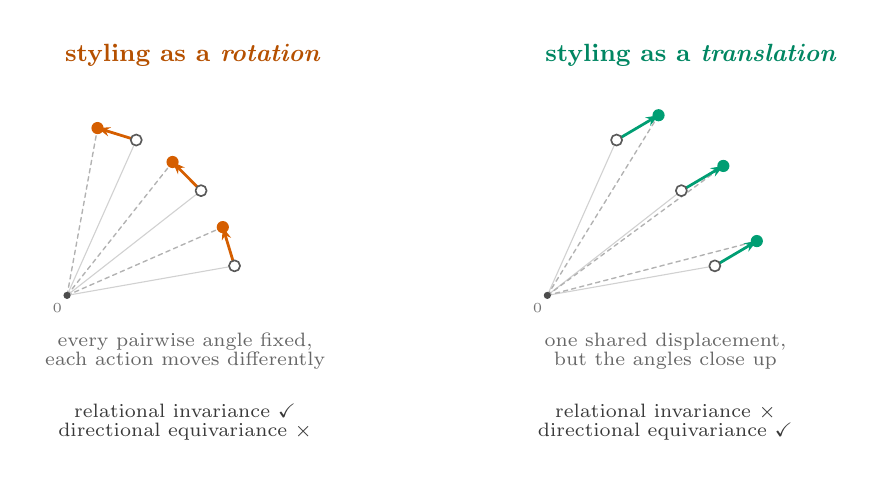
\begin{tikzpicture}[font=\small,line cap=round,line join=round,x=1cm,y=1cm]
\useasboundingbox (-0.5,-2.05) rectangle (10.05,3.4);
\begin{scope}[shift={(0.0,0)}]
\node[font=\small\bfseries,text=okverm!85!black,anchor=west] at (-0.15,3.05) {styling as a \emph{rotation}};
\draw[black!18,line width=0.4pt] (0,0) -- (2.127,0.375);
\draw[black!30,line width=0.5pt,dash pattern=on 1.6pt off 1.4pt] (0,0) -- (1.978,0.867);
\draw[-{Stealth[length=4.5pt,width=3.4pt]},okverm,line width=1.0pt] (2.127,0.375) -- (1.978,0.867);
\node[circle,draw=black!65,fill=white,inner sep=0pt,minimum size=4pt,line width=0.6pt] at (2.127,0.375) {};
\node[circle,fill=okverm,inner sep=0pt,minimum size=4.4pt] at (1.978,0.867) {};
\draw[black!18,line width=0.4pt] (0,0) -- (1.702,1.330);
\draw[black!30,line width=0.5pt,dash pattern=on 1.6pt off 1.4pt] (0,0) -- (1.340,1.694);
\draw[-{Stealth[length=4.5pt,width=3.4pt]},okverm,line width=1.0pt] (1.702,1.330) -- (1.340,1.694);
\node[circle,draw=black!65,fill=white,inner sep=0pt,minimum size=4pt,line width=0.6pt] at (1.702,1.330) {};
\node[circle,fill=okverm,inner sep=0pt,minimum size=4.4pt] at (1.340,1.694) {};
\draw[black!18,line width=0.4pt] (0,0) -- (0.879,1.973);
\draw[black!30,line width=0.5pt,dash pattern=on 1.6pt off 1.4pt] (0,0) -- (0.387,2.125);
\draw[-{Stealth[length=4.5pt,width=3.4pt]},okverm,line width=1.0pt] (0.879,1.973) -- (0.387,2.125);
\node[circle,draw=black!65,fill=white,inner sep=0pt,minimum size=4pt,line width=0.6pt] at (0.879,1.973) {};
\node[circle,fill=okverm,inner sep=0pt,minimum size=4.4pt] at (0.387,2.125) {};
\fill[black!70] (0,0) circle (1.3pt);
\node[font=\tiny,text=black!55,anchor=north east] at (0.06,0.02) {$0$};
\node[font=\scriptsize,text=black!60,align=center,anchor=north] at (1.5,-0.35) {every pairwise angle fixed,\\[-1pt] each action moves differently};
\node[font=\scriptsize,text=black!78,align=center,anchor=north] at (1.5,-1.25) {relational invariance \checkmark\\[-1pt] directional equivariance $\times$};
\end{scope}
\begin{scope}[shift={(6.1,0)}]
\node[font=\small\bfseries,text=okgreen!85!black,anchor=west] at (-0.15,3.05) {styling as a \emph{translation}};
\draw[black!18,line width=0.4pt] (0,0) -- (2.127,0.375);
\draw[black!30,line width=0.5pt,dash pattern=on 1.6pt off 1.4pt] (0,0) -- (2.660,0.690);
\draw[-{Stealth[length=4.5pt,width=3.4pt]},okgreen,line width=1.0pt] (2.127,0.375) -- (2.660,0.690);
\node[circle,draw=black!65,fill=white,inner sep=0pt,minimum size=4pt,line width=0.6pt] at (2.127,0.375) {};
\node[circle,fill=okgreen,inner sep=0pt,minimum size=4.4pt] at (2.660,0.690) {};
\draw[black!18,line width=0.4pt] (0,0) -- (1.702,1.330);
\draw[black!30,line width=0.5pt,dash pattern=on 1.6pt off 1.4pt] (0,0) -- (2.235,1.644);
\draw[-{Stealth[length=4.5pt,width=3.4pt]},okgreen,line width=1.0pt] (1.702,1.330) -- (2.235,1.644);
\node[circle,draw=black!65,fill=white,inner sep=0pt,minimum size=4pt,line width=0.6pt] at (1.702,1.330) {};
\node[circle,fill=okgreen,inner sep=0pt,minimum size=4.4pt] at (2.235,1.644) {};
\draw[black!18,line width=0.4pt] (0,0) -- (0.879,1.973);
\draw[black!30,line width=0.5pt,dash pattern=on 1.6pt off 1.4pt] (0,0) -- (1.412,2.288);
\draw[-{Stealth[length=4.5pt,width=3.4pt]},okgreen,line width=1.0pt] (0.879,1.973) -- (1.412,2.288);
\node[circle,draw=black!65,fill=white,inner sep=0pt,minimum size=4pt,line width=0.6pt] at (0.879,1.973) {};
\node[circle,fill=okgreen,inner sep=0pt,minimum size=4.4pt] at (1.412,2.288) {};
\fill[black!70] (0,0) circle (1.3pt);
\node[font=\tiny,text=black!55,anchor=north east] at (0.06,0.02) {$0$};
\node[font=\scriptsize,text=black!60,align=center,anchor=north] at (1.5,-0.35) {one shared displacement,\\[-1pt] but the angles close up};
\node[font=\scriptsize,text=black!78,align=center,anchor=north] at (1.5,-1.25) {relational invariance $\times$\\[-1pt] directional equivariance \checkmark};
\end{scope}
\end{tikzpicture}
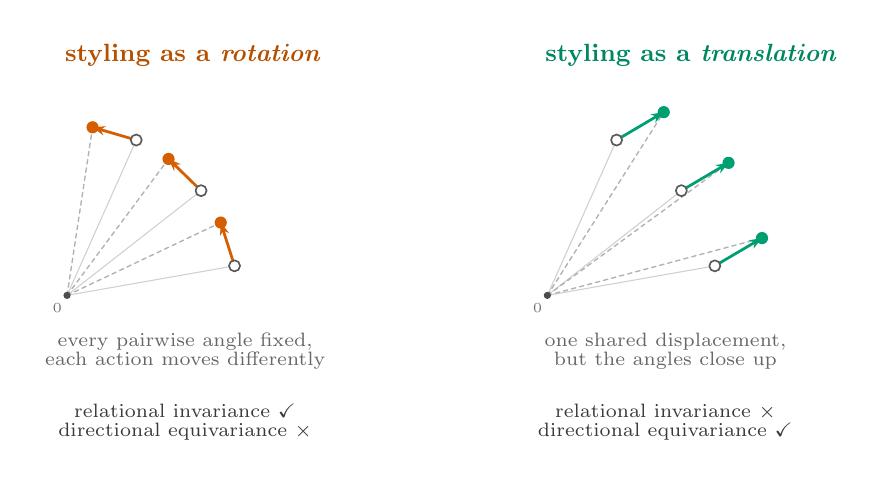
\begin{tikzpicture}[font=\small,line cap=round,line join=round,x=1cm,y=1cm]
\useasboundingbox (-0.5,-2.05) rectangle (10.05,3.4);
\begin{scope}[shift={(0.0,0)}]
\node[font=\small\bfseries,text=okverm!85!black,anchor=west] at (-0.15,3.05) {styling as a \emph{rotation}};
\draw[black!18,line width=0.4pt] (0,0) -- (2.127,0.375);
\draw[black!30,line width=0.5pt,dash pattern=on 1.6pt off 1.4pt] (0,0) -- (1.952,0.925);
\draw[-{Stealth[length=4.5pt,width=3.4pt]},okverm,line width=1.0pt] (2.127,0.375) -- (1.952,0.925);
\node[circle,draw=black!65,fill=white,inner sep=0pt,minimum size=4pt,line width=0.6pt] at (2.127,0.375) {};
\node[circle,fill=okverm,inner sep=0pt,minimum size=4.4pt] at (1.952,0.925) {};
\draw[black!18,line width=0.4pt] (0,0) -- (1.702,1.330);
\draw[black!30,line width=0.5pt,dash pattern=on 1.6pt off 1.4pt] (0,0) -- (1.289,1.733);
\draw[-{Stealth[length=4.5pt,width=3.4pt]},okverm,line width=1.0pt] (1.702,1.330) -- (1.289,1.733);
\node[circle,draw=black!65,fill=white,inner sep=0pt,minimum size=4pt,line width=0.6pt] at (1.702,1.330) {};
\node[circle,fill=okverm,inner sep=0pt,minimum size=4.4pt] at (1.289,1.733) {};
\draw[black!18,line width=0.4pt] (0,0) -- (0.879,1.973);
\draw[black!30,line width=0.5pt,dash pattern=on 1.6pt off 1.4pt] (0,0) -- (0.324,2.135);
\draw[-{Stealth[length=4.5pt,width=3.4pt]},okverm,line width=1.0pt] (0.879,1.973) -- (0.324,2.135);
\node[circle,draw=black!65,fill=white,inner sep=0pt,minimum size=4pt,line width=0.6pt] at (0.879,1.973) {};
\node[circle,fill=okverm,inner sep=0pt,minimum size=4.4pt] at (0.324,2.135) {};
\fill[black!70] (0,0) circle (1.3pt);
\node[font=\tiny,text=black!55,anchor=north east] at (0.06,0.02) {$0$};
\node[font=\scriptsize,text=black!60,align=center,anchor=north] at (1.5,-0.35) {every pairwise angle fixed,\\[-1pt] each action moves differently};
\node[font=\scriptsize,text=black!78,align=center,anchor=north] at (1.5,-1.25) {relational invariance \checkmark\\[-1pt] directional equivariance $\times$};
\end{scope}
\begin{scope}[shift={(6.1,0)}]
\node[font=\small\bfseries,text=okgreen!85!black,anchor=west] at (-0.15,3.05) {styling as a \emph{translation}};
\draw[black!18,line width=0.4pt] (0,0) -- (2.127,0.375);
\draw[black!30,line width=0.5pt,dash pattern=on 1.6pt off 1.4pt] (0,0) -- (2.726,0.728);
\draw[-{Stealth[length=4.5pt,width=3.4pt]},okgreen,line width=1.0pt] (2.127,0.375) -- (2.726,0.728);
\node[circle,draw=black!65,fill=white,inner sep=0pt,minimum size=4pt,line width=0.6pt] at (2.127,0.375) {};
\node[circle,fill=okgreen,inner sep=0pt,minimum size=4.4pt] at (2.726,0.728) {};
\draw[black!18,line width=0.4pt] (0,0) -- (1.702,1.330);
\draw[black!30,line width=0.5pt,dash pattern=on 1.6pt off 1.4pt] (0,0) -- (2.301,1.683);
\draw[-{Stealth[length=4.5pt,width=3.4pt]},okgreen,line width=1.0pt] (1.702,1.330) -- (2.301,1.683);
\node[circle,draw=black!65,fill=white,inner sep=0pt,minimum size=4pt,line width=0.6pt] at (1.702,1.330) {};
\node[circle,fill=okgreen,inner sep=0pt,minimum size=4.4pt] at (2.301,1.683) {};
\draw[black!18,line width=0.4pt] (0,0) -- (0.879,1.973);
\draw[black!30,line width=0.5pt,dash pattern=on 1.6pt off 1.4pt] (0,0) -- (1.478,2.327);
\draw[-{Stealth[length=4.5pt,width=3.4pt]},okgreen,line width=1.0pt] (0.879,1.973) -- (1.478,2.327);
\node[circle,draw=black!65,fill=white,inner sep=0pt,minimum size=4pt,line width=0.6pt] at (0.879,1.973) {};
\node[circle,fill=okgreen,inner sep=0pt,minimum size=4.4pt] at (1.478,2.327) {};
\fill[black!70] (0,0) circle (1.3pt);
\node[font=\tiny,text=black!55,anchor=north east] at (0.06,0.02) {$0$};
\node[font=\scriptsize,text=black!60,align=center,anchor=north] at (1.5,-0.35) {one shared displacement,\\[-1pt] but the angles close up};
\node[font=\scriptsize,text=black!78,align=center,anchor=north] at (1.5,-1.25) {relational invariance $\times$\\[-1pt] directional equivariance \checkmark};
\end{scope}
\end{tikzpicture}
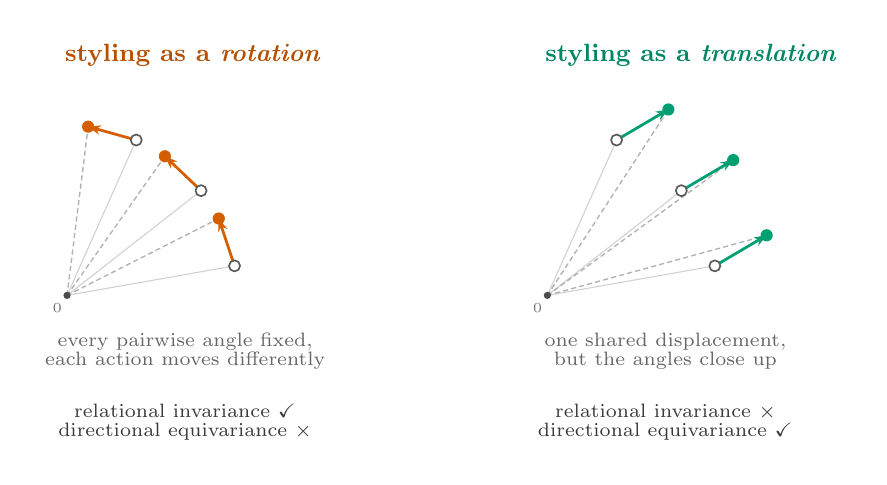
\begin{tikzpicture}[font=\small,line cap=round,line join=round,x=1cm,y=1cm]
\useasboundingbox (-0.5,-2.05) rectangle (10.05,3.4);
\begin{scope}[shift={(0.0,0)}]
\node[font=\small\bfseries,text=okverm!85!black,anchor=west] at (-0.15,3.05) {styling as a \emph{rotation}};
\draw[black!18,line width=0.4pt] (0,0) -- (2.127,0.375);
\draw[black!30,line width=0.5pt,dash pattern=on 1.6pt off 1.4pt] (0,0) -- (1.927,0.976);
\draw[-{Stealth[length=4.5pt,width=3.4pt]},okverm,line width=1.0pt] (2.127,0.375) -- (1.927,0.976);
\node[circle,draw=black!65,fill=white,inner sep=0pt,minimum size=4pt,line width=0.6pt] at (2.127,0.375) {};
\node[circle,fill=okverm,inner sep=0pt,minimum size=4.4pt] at (1.927,0.976) {};
\draw[black!18,line width=0.4pt] (0,0) -- (1.702,1.330);
\draw[black!30,line width=0.5pt,dash pattern=on 1.6pt off 1.4pt] (0,0) -- (1.243,1.767);
\draw[-{Stealth[length=4.5pt,width=3.4pt]},okverm,line width=1.0pt] (1.702,1.330) -- (1.243,1.767);
\node[circle,draw=black!65,fill=white,inner sep=0pt,minimum size=4pt,line width=0.6pt] at (1.702,1.330) {};
\node[circle,fill=okverm,inner sep=0pt,minimum size=4.4pt] at (1.243,1.767) {};
\draw[black!18,line width=0.4pt] (0,0) -- (0.879,1.973);
\draw[black!30,line width=0.5pt,dash pattern=on 1.6pt off 1.4pt] (0,0) -- (0.268,2.143);
\draw[-{Stealth[length=4.5pt,width=3.4pt]},okverm,line width=1.0pt] (0.879,1.973) -- (0.268,2.143);
\node[circle,draw=black!65,fill=white,inner sep=0pt,minimum size=4pt,line width=0.6pt] at (0.879,1.973) {};
\node[circle,fill=okverm,inner sep=0pt,minimum size=4.4pt] at (0.268,2.143) {};
\fill[black!70] (0,0) circle (1.3pt);
\node[font=\tiny,text=black!55,anchor=north east] at (0.06,0.02) {$0$};
\node[font=\scriptsize,text=black!60,align=center,anchor=north] at (1.5,-0.35) {every pairwise angle fixed,\\[-1pt] each action moves differently};
\node[font=\scriptsize,text=black!78,align=center,anchor=north] at (1.5,-1.25) {relational invariance \checkmark\\[-1pt] directional equivariance $\times$};
\end{scope}
\begin{scope}[shift={(6.1,0)}]
\node[font=\small\bfseries,text=okgreen!85!black,anchor=west] at (-0.15,3.05) {styling as a \emph{translation}};
\draw[black!18,line width=0.4pt] (0,0) -- (2.127,0.375);
\draw[black!30,line width=0.5pt,dash pattern=on 1.6pt off 1.4pt] (0,0) -- (2.785,0.763);
\draw[-{Stealth[length=4.5pt,width=3.4pt]},okgreen,line width=1.0pt] (2.127,0.375) -- (2.785,0.763);
\node[circle,draw=black!65,fill=white,inner sep=0pt,minimum size=4pt,line width=0.6pt] at (2.127,0.375) {};
\node[circle,fill=okgreen,inner sep=0pt,minimum size=4.4pt] at (2.785,0.763) {};
\draw[black!18,line width=0.4pt] (0,0) -- (1.702,1.330);
\draw[black!30,line width=0.5pt,dash pattern=on 1.6pt off 1.4pt] (0,0) -- (2.360,1.718);
\draw[-{Stealth[length=4.5pt,width=3.4pt]},okgreen,line width=1.0pt] (1.702,1.330) -- (2.360,1.718);
\node[circle,draw=black!65,fill=white,inner sep=0pt,minimum size=4pt,line width=0.6pt] at (1.702,1.330) {};
\node[circle,fill=okgreen,inner sep=0pt,minimum size=4.4pt] at (2.360,1.718) {};
\draw[black!18,line width=0.4pt] (0,0) -- (0.879,1.973);
\draw[black!30,line width=0.5pt,dash pattern=on 1.6pt off 1.4pt] (0,0) -- (1.537,2.361);
\draw[-{Stealth[length=4.5pt,width=3.4pt]},okgreen,line width=1.0pt] (0.879,1.973) -- (1.537,2.361);
\node[circle,draw=black!65,fill=white,inner sep=0pt,minimum size=4pt,line width=0.6pt] at (0.879,1.973) {};
\node[circle,fill=okgreen,inner sep=0pt,minimum size=4.4pt] at (1.537,2.361) {};
\fill[black!70] (0,0) circle (1.3pt);
\node[font=\tiny,text=black!55,anchor=north east] at (0.06,0.02) {$0$};
\node[font=\scriptsize,text=black!60,align=center,anchor=north] at (1.5,-0.35) {one shared displacement,\\[-1pt] but the angles close up};
\node[font=\scriptsize,text=black!78,align=center,anchor=north] at (1.5,-1.25) {relational invariance $\times$\\[-1pt] directional equivariance \checkmark};
\end{scope}
\end{tikzpicture}
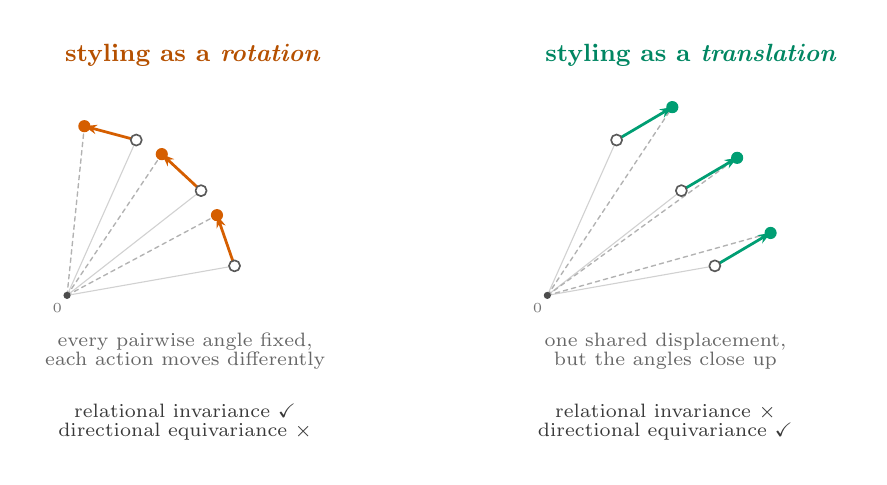
\begin{tikzpicture}[font=\small,line cap=round,line join=round,x=1cm,y=1cm]
\useasboundingbox (-0.5,-2.05) rectangle (10.05,3.4);
\begin{scope}[shift={(0.0,0)}]
\node[font=\small\bfseries,text=okverm!85!black,anchor=west] at (-0.15,3.05) {styling as a \emph{rotation}};
\draw[black!18,line width=0.4pt] (0,0) -- (2.127,0.375);
\draw[black!30,line width=0.5pt,dash pattern=on 1.6pt off 1.4pt] (0,0) -- (1.904,1.019);
\draw[-{Stealth[length=4.5pt,width=3.4pt]},okverm,line width=1.0pt] (2.127,0.375) -- (1.904,1.019);
\node[circle,draw=black!65,fill=white,inner sep=0pt,minimum size=4pt,line width=0.6pt] at (2.127,0.375) {};
\node[circle,fill=okverm,inner sep=0pt,minimum size=4.4pt] at (1.904,1.019) {};
\draw[black!18,line width=0.4pt] (0,0) -- (1.702,1.330);
\draw[black!30,line width=0.5pt,dash pattern=on 1.6pt off 1.4pt] (0,0) -- (1.203,1.794);
\draw[-{Stealth[length=4.5pt,width=3.4pt]},okverm,line width=1.0pt] (1.702,1.330) -- (1.203,1.794);
\node[circle,draw=black!65,fill=white,inner sep=0pt,minimum size=4pt,line width=0.6pt] at (1.702,1.330) {};
\node[circle,fill=okverm,inner sep=0pt,minimum size=4.4pt] at (1.203,1.794) {};
\draw[black!18,line width=0.4pt] (0,0) -- (0.879,1.973);
\draw[black!30,line width=0.5pt,dash pattern=on 1.6pt off 1.4pt] (0,0) -- (0.220,2.149);
\draw[-{Stealth[length=4.5pt,width=3.4pt]},okverm,line width=1.0pt] (0.879,1.973) -- (0.220,2.149);
\node[circle,draw=black!65,fill=white,inner sep=0pt,minimum size=4pt,line width=0.6pt] at (0.879,1.973) {};
\node[circle,fill=okverm,inner sep=0pt,minimum size=4.4pt] at (0.220,2.149) {};
\fill[black!70] (0,0) circle (1.3pt);
\node[font=\tiny,text=black!55,anchor=north east] at (0.06,0.02) {$0$};
\node[font=\scriptsize,text=black!60,align=center,anchor=north] at (1.5,-0.35) {every pairwise angle fixed,\\[-1pt] each action moves differently};
\node[font=\scriptsize,text=black!78,align=center,anchor=north] at (1.5,-1.25) {relational invariance \checkmark\\[-1pt] directional equivariance $\times$};
\end{scope}
\begin{scope}[shift={(6.1,0)}]
\node[font=\small\bfseries,text=okgreen!85!black,anchor=west] at (-0.15,3.05) {styling as a \emph{translation}};
\draw[black!18,line width=0.4pt] (0,0) -- (2.127,0.375);
\draw[black!30,line width=0.5pt,dash pattern=on 1.6pt off 1.4pt] (0,0) -- (2.835,0.793);
\draw[-{Stealth[length=4.5pt,width=3.4pt]},okgreen,line width=1.0pt] (2.127,0.375) -- (2.835,0.793);
\node[circle,draw=black!65,fill=white,inner sep=0pt,minimum size=4pt,line width=0.6pt] at (2.127,0.375) {};
\node[circle,fill=okgreen,inner sep=0pt,minimum size=4.4pt] at (2.835,0.793) {};
\draw[black!18,line width=0.4pt] (0,0) -- (1.702,1.330);
\draw[black!30,line width=0.5pt,dash pattern=on 1.6pt off 1.4pt] (0,0) -- (2.410,1.747);
\draw[-{Stealth[length=4.5pt,width=3.4pt]},okgreen,line width=1.0pt] (1.702,1.330) -- (2.410,1.747);
\node[circle,draw=black!65,fill=white,inner sep=0pt,minimum size=4pt,line width=0.6pt] at (1.702,1.330) {};
\node[circle,fill=okgreen,inner sep=0pt,minimum size=4.4pt] at (2.410,1.747) {};
\draw[black!18,line width=0.4pt] (0,0) -- (0.879,1.973);
\draw[black!30,line width=0.5pt,dash pattern=on 1.6pt off 1.4pt] (0,0) -- (1.587,2.391);
\draw[-{Stealth[length=4.5pt,width=3.4pt]},okgreen,line width=1.0pt] (0.879,1.973) -- (1.587,2.391);
\node[circle,draw=black!65,fill=white,inner sep=0pt,minimum size=4pt,line width=0.6pt] at (0.879,1.973) {};
\node[circle,fill=okgreen,inner sep=0pt,minimum size=4.4pt] at (1.587,2.391) {};
\fill[black!70] (0,0) circle (1.3pt);
\node[font=\tiny,text=black!55,anchor=north east] at (0.06,0.02) {$0$};
\node[font=\scriptsize,text=black!60,align=center,anchor=north] at (1.5,-0.35) {one shared displacement,\\[-1pt] but the angles close up};
\node[font=\scriptsize,text=black!78,align=center,anchor=north] at (1.5,-1.25) {relational invariance $\times$\\[-1pt] directional equivariance \checkmark};
\end{scope}
\end{tikzpicture}
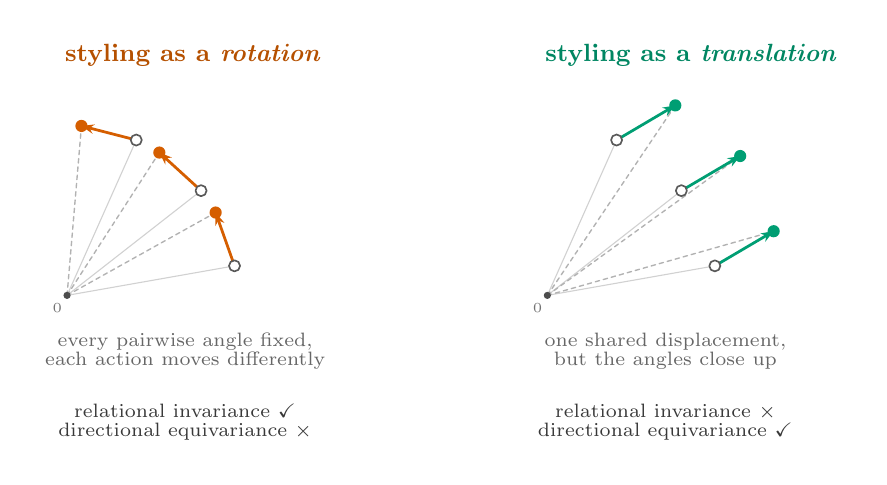
\begin{tikzpicture}[font=\small,line cap=round,line join=round,x=1cm,y=1cm]
\useasboundingbox (-0.5,-2.05) rectangle (10.05,3.4);
\begin{scope}[shift={(0.0,0)}]
\node[font=\small\bfseries,text=okverm!85!black,anchor=west] at (-0.15,3.05) {styling as a \emph{rotation}};
\draw[black!18,line width=0.4pt] (0,0) -- (2.127,0.375);
\draw[black!30,line width=0.5pt,dash pattern=on 1.6pt off 1.4pt] (0,0) -- (1.887,1.052);
\draw[-{Stealth[length=4.5pt,width=3.4pt]},okverm,line width=1.0pt] (2.127,0.375) -- (1.887,1.052);
\node[circle,draw=black!65,fill=white,inner sep=0pt,minimum size=4pt,line width=0.6pt] at (2.127,0.375) {};
\node[circle,fill=okverm,inner sep=0pt,minimum size=4.4pt] at (1.887,1.052) {};
\draw[black!18,line width=0.4pt] (0,0) -- (1.702,1.330);
\draw[black!30,line width=0.5pt,dash pattern=on 1.6pt off 1.4pt] (0,0) -- (1.172,1.814);
\draw[-{Stealth[length=4.5pt,width=3.4pt]},okverm,line width=1.0pt] (1.702,1.330) -- (1.172,1.814);
\node[circle,draw=black!65,fill=white,inner sep=0pt,minimum size=4pt,line width=0.6pt] at (1.702,1.330) {};
\node[circle,fill=okverm,inner sep=0pt,minimum size=4.4pt] at (1.172,1.814) {};
\draw[black!18,line width=0.4pt] (0,0) -- (0.879,1.973);
\draw[black!30,line width=0.5pt,dash pattern=on 1.6pt off 1.4pt] (0,0) -- (0.183,2.152);
\draw[-{Stealth[length=4.5pt,width=3.4pt]},okverm,line width=1.0pt] (0.879,1.973) -- (0.183,2.152);
\node[circle,draw=black!65,fill=white,inner sep=0pt,minimum size=4pt,line width=0.6pt] at (0.879,1.973) {};
\node[circle,fill=okverm,inner sep=0pt,minimum size=4.4pt] at (0.183,2.152) {};
\fill[black!70] (0,0) circle (1.3pt);
\node[font=\tiny,text=black!55,anchor=north east] at (0.06,0.02) {$0$};
\node[font=\scriptsize,text=black!60,align=center,anchor=north] at (1.5,-0.35) {every pairwise angle fixed,\\[-1pt] each action moves differently};
\node[font=\scriptsize,text=black!78,align=center,anchor=north] at (1.5,-1.25) {relational invariance \checkmark\\[-1pt] directional equivariance $\times$};
\end{scope}
\begin{scope}[shift={(6.1,0)}]
\node[font=\small\bfseries,text=okgreen!85!black,anchor=west] at (-0.15,3.05) {styling as a \emph{translation}};
\draw[black!18,line width=0.4pt] (0,0) -- (2.127,0.375);
\draw[black!30,line width=0.5pt,dash pattern=on 1.6pt off 1.4pt] (0,0) -- (2.874,0.815);
\draw[-{Stealth[length=4.5pt,width=3.4pt]},okgreen,line width=1.0pt] (2.127,0.375) -- (2.874,0.815);
\node[circle,draw=black!65,fill=white,inner sep=0pt,minimum size=4pt,line width=0.6pt] at (2.127,0.375) {};
\node[circle,fill=okgreen,inner sep=0pt,minimum size=4.4pt] at (2.874,0.815) {};
\draw[black!18,line width=0.4pt] (0,0) -- (1.702,1.330);
\draw[black!30,line width=0.5pt,dash pattern=on 1.6pt off 1.4pt] (0,0) -- (2.449,1.770);
\draw[-{Stealth[length=4.5pt,width=3.4pt]},okgreen,line width=1.0pt] (1.702,1.330) -- (2.449,1.770);
\node[circle,draw=black!65,fill=white,inner sep=0pt,minimum size=4pt,line width=0.6pt] at (1.702,1.330) {};
\node[circle,fill=okgreen,inner sep=0pt,minimum size=4.4pt] at (2.449,1.770) {};
\draw[black!18,line width=0.4pt] (0,0) -- (0.879,1.973);
\draw[black!30,line width=0.5pt,dash pattern=on 1.6pt off 1.4pt] (0,0) -- (1.625,2.413);
\draw[-{Stealth[length=4.5pt,width=3.4pt]},okgreen,line width=1.0pt] (0.879,1.973) -- (1.625,2.413);
\node[circle,draw=black!65,fill=white,inner sep=0pt,minimum size=4pt,line width=0.6pt] at (0.879,1.973) {};
\node[circle,fill=okgreen,inner sep=0pt,minimum size=4.4pt] at (1.625,2.413) {};
\fill[black!70] (0,0) circle (1.3pt);
\node[font=\tiny,text=black!55,anchor=north east] at (0.06,0.02) {$0$};
\node[font=\scriptsize,text=black!60,align=center,anchor=north] at (1.5,-0.35) {one shared displacement,\\[-1pt] but the angles close up};
\node[font=\scriptsize,text=black!78,align=center,anchor=north] at (1.5,-1.25) {relational invariance $\times$\\[-1pt] directional equivariance \checkmark};
\end{scope}
\end{tikzpicture}
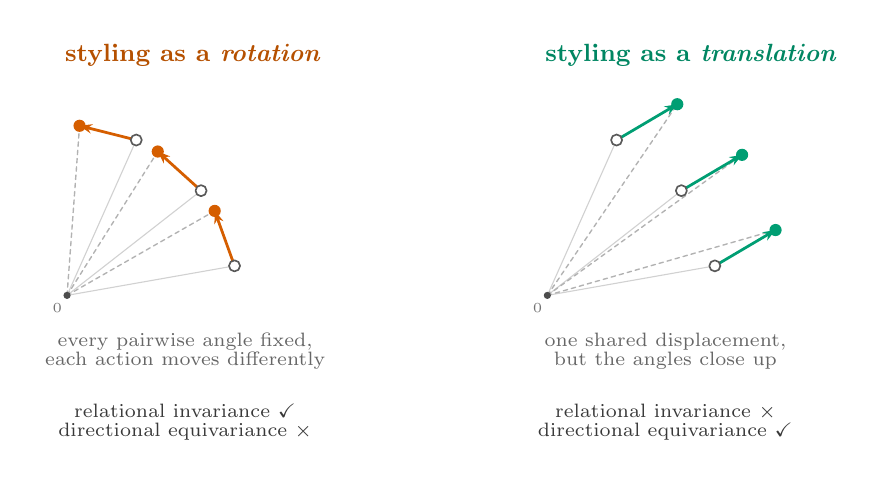
\begin{tikzpicture}[font=\small,line cap=round,line join=round,x=1cm,y=1cm]
\useasboundingbox (-0.5,-2.05) rectangle (10.05,3.4);
\begin{scope}[shift={(0.0,0)}]
\node[font=\small\bfseries,text=okverm!85!black,anchor=west] at (-0.15,3.05) {styling as a \emph{rotation}};
\draw[black!18,line width=0.4pt] (0,0) -- (2.127,0.375);
\draw[black!30,line width=0.5pt,dash pattern=on 1.6pt off 1.4pt] (0,0) -- (1.875,1.073);
\draw[-{Stealth[length=4.5pt,width=3.4pt]},okverm,line width=1.0pt] (2.127,0.375) -- (1.875,1.073);
\node[circle,draw=black!65,fill=white,inner sep=0pt,minimum size=4pt,line width=0.6pt] at (2.127,0.375) {};
\node[circle,fill=okverm,inner sep=0pt,minimum size=4.4pt] at (1.875,1.073) {};
\draw[black!18,line width=0.4pt] (0,0) -- (1.702,1.330);
\draw[black!30,line width=0.5pt,dash pattern=on 1.6pt off 1.4pt] (0,0) -- (1.152,1.827);
\draw[-{Stealth[length=4.5pt,width=3.4pt]},okverm,line width=1.0pt] (1.702,1.330) -- (1.152,1.827);
\node[circle,draw=black!65,fill=white,inner sep=0pt,minimum size=4pt,line width=0.6pt] at (1.702,1.330) {};
\node[circle,fill=okverm,inner sep=0pt,minimum size=4.4pt] at (1.152,1.827) {};
\draw[black!18,line width=0.4pt] (0,0) -- (0.879,1.973);
\draw[black!30,line width=0.5pt,dash pattern=on 1.6pt off 1.4pt] (0,0) -- (0.159,2.154);
\draw[-{Stealth[length=4.5pt,width=3.4pt]},okverm,line width=1.0pt] (0.879,1.973) -- (0.159,2.154);
\node[circle,draw=black!65,fill=white,inner sep=0pt,minimum size=4pt,line width=0.6pt] at (0.879,1.973) {};
\node[circle,fill=okverm,inner sep=0pt,minimum size=4.4pt] at (0.159,2.154) {};
\fill[black!70] (0,0) circle (1.3pt);
\node[font=\tiny,text=black!55,anchor=north east] at (0.06,0.02) {$0$};
\node[font=\scriptsize,text=black!60,align=center,anchor=north] at (1.5,-0.35) {every pairwise angle fixed,\\[-1pt] each action moves differently};
\node[font=\scriptsize,text=black!78,align=center,anchor=north] at (1.5,-1.25) {relational invariance \checkmark\\[-1pt] directional equivariance $\times$};
\end{scope}
\begin{scope}[shift={(6.1,0)}]
\node[font=\small\bfseries,text=okgreen!85!black,anchor=west] at (-0.15,3.05) {styling as a \emph{translation}};
\draw[black!18,line width=0.4pt] (0,0) -- (2.127,0.375);
\draw[black!30,line width=0.5pt,dash pattern=on 1.6pt off 1.4pt] (0,0) -- (2.898,0.830);
\draw[-{Stealth[length=4.5pt,width=3.4pt]},okgreen,line width=1.0pt] (2.127,0.375) -- (2.898,0.830);
\node[circle,draw=black!65,fill=white,inner sep=0pt,minimum size=4pt,line width=0.6pt] at (2.127,0.375) {};
\node[circle,fill=okgreen,inner sep=0pt,minimum size=4.4pt] at (2.898,0.830) {};
\draw[black!18,line width=0.4pt] (0,0) -- (1.702,1.330);
\draw[black!30,line width=0.5pt,dash pattern=on 1.6pt off 1.4pt] (0,0) -- (2.473,1.785);
\draw[-{Stealth[length=4.5pt,width=3.4pt]},okgreen,line width=1.0pt] (1.702,1.330) -- (2.473,1.785);
\node[circle,draw=black!65,fill=white,inner sep=0pt,minimum size=4pt,line width=0.6pt] at (1.702,1.330) {};
\node[circle,fill=okgreen,inner sep=0pt,minimum size=4.4pt] at (2.473,1.785) {};
\draw[black!18,line width=0.4pt] (0,0) -- (0.879,1.973);
\draw[black!30,line width=0.5pt,dash pattern=on 1.6pt off 1.4pt] (0,0) -- (1.650,2.428);
\draw[-{Stealth[length=4.5pt,width=3.4pt]},okgreen,line width=1.0pt] (0.879,1.973) -- (1.650,2.428);
\node[circle,draw=black!65,fill=white,inner sep=0pt,minimum size=4pt,line width=0.6pt] at (0.879,1.973) {};
\node[circle,fill=okgreen,inner sep=0pt,minimum size=4.4pt] at (1.650,2.428) {};
\fill[black!70] (0,0) circle (1.3pt);
\node[font=\tiny,text=black!55,anchor=north east] at (0.06,0.02) {$0$};
\node[font=\scriptsize,text=black!60,align=center,anchor=north] at (1.5,-0.35) {one shared displacement,\\[-1pt] but the angles close up};
\node[font=\scriptsize,text=black!78,align=center,anchor=north] at (1.5,-1.25) {relational invariance $\times$\\[-1pt] directional equivariance \checkmark};
\end{scope}
\end{tikzpicture}
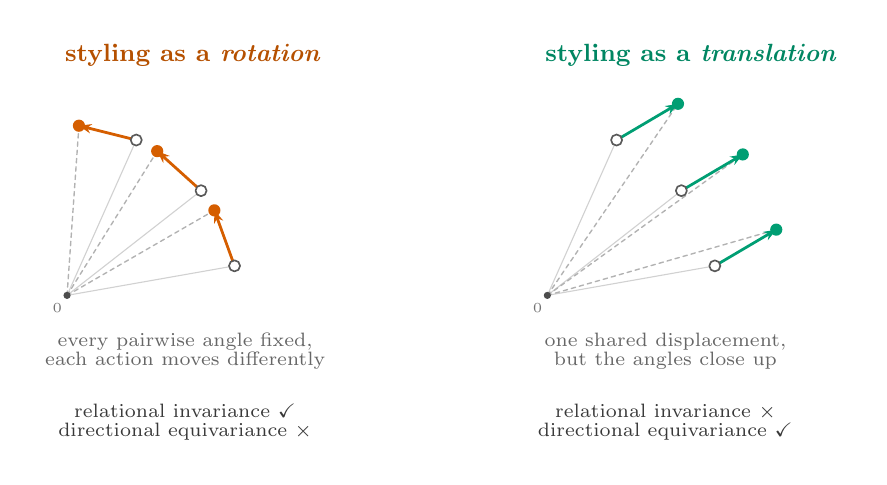
\begin{tikzpicture}[font=\small,line cap=round,line join=round,x=1cm,y=1cm]
\useasboundingbox (-0.5,-2.05) rectangle (10.05,3.4);
\begin{scope}[shift={(0.0,0)}]
\node[font=\small\bfseries,text=okverm!85!black,anchor=west] at (-0.15,3.05) {styling as a \emph{rotation}};
\draw[black!18,line width=0.4pt] (0,0) -- (2.127,0.375);
\draw[black!30,line width=0.5pt,dash pattern=on 1.6pt off 1.4pt] (0,0) -- (1.871,1.080);
\draw[-{Stealth[length=4.5pt,width=3.4pt]},okverm,line width=1.0pt] (2.127,0.375) -- (1.871,1.080);
\node[circle,draw=black!65,fill=white,inner sep=0pt,minimum size=4pt,line width=0.6pt] at (2.127,0.375) {};
\node[circle,fill=okverm,inner sep=0pt,minimum size=4.4pt] at (1.871,1.080) {};
\draw[black!18,line width=0.4pt] (0,0) -- (1.702,1.330);
\draw[black!30,line width=0.5pt,dash pattern=on 1.6pt off 1.4pt] (0,0) -- (1.145,1.832);
\draw[-{Stealth[length=4.5pt,width=3.4pt]},okverm,line width=1.0pt] (1.702,1.330) -- (1.145,1.832);
\node[circle,draw=black!65,fill=white,inner sep=0pt,minimum size=4pt,line width=0.6pt] at (1.702,1.330) {};
\node[circle,fill=okverm,inner sep=0pt,minimum size=4.4pt] at (1.145,1.832) {};
\draw[black!18,line width=0.4pt] (0,0) -- (0.879,1.973);
\draw[black!30,line width=0.5pt,dash pattern=on 1.6pt off 1.4pt] (0,0) -- (0.151,2.155);
\draw[-{Stealth[length=4.5pt,width=3.4pt]},okverm,line width=1.0pt] (0.879,1.973) -- (0.151,2.155);
\node[circle,draw=black!65,fill=white,inner sep=0pt,minimum size=4pt,line width=0.6pt] at (0.879,1.973) {};
\node[circle,fill=okverm,inner sep=0pt,minimum size=4.4pt] at (0.151,2.155) {};
\fill[black!70] (0,0) circle (1.3pt);
\node[font=\tiny,text=black!55,anchor=north east] at (0.06,0.02) {$0$};
\node[font=\scriptsize,text=black!60,align=center,anchor=north] at (1.5,-0.35) {every pairwise angle fixed,\\[-1pt] each action moves differently};
\node[font=\scriptsize,text=black!78,align=center,anchor=north] at (1.5,-1.25) {relational invariance \checkmark\\[-1pt] directional equivariance $\times$};
\end{scope}
\begin{scope}[shift={(6.1,0)}]
\node[font=\small\bfseries,text=okgreen!85!black,anchor=west] at (-0.15,3.05) {styling as a \emph{translation}};
\draw[black!18,line width=0.4pt] (0,0) -- (2.127,0.375);
\draw[black!30,line width=0.5pt,dash pattern=on 1.6pt off 1.4pt] (0,0) -- (2.907,0.835);
\draw[-{Stealth[length=4.5pt,width=3.4pt]},okgreen,line width=1.0pt] (2.127,0.375) -- (2.907,0.835);
\node[circle,draw=black!65,fill=white,inner sep=0pt,minimum size=4pt,line width=0.6pt] at (2.127,0.375) {};
\node[circle,fill=okgreen,inner sep=0pt,minimum size=4.4pt] at (2.907,0.835) {};
\draw[black!18,line width=0.4pt] (0,0) -- (1.702,1.330);
\draw[black!30,line width=0.5pt,dash pattern=on 1.6pt off 1.4pt] (0,0) -- (2.482,1.790);
\draw[-{Stealth[length=4.5pt,width=3.4pt]},okgreen,line width=1.0pt] (1.702,1.330) -- (2.482,1.790);
\node[circle,draw=black!65,fill=white,inner sep=0pt,minimum size=4pt,line width=0.6pt] at (1.702,1.330) {};
\node[circle,fill=okgreen,inner sep=0pt,minimum size=4.4pt] at (2.482,1.790) {};
\draw[black!18,line width=0.4pt] (0,0) -- (0.879,1.973);
\draw[black!30,line width=0.5pt,dash pattern=on 1.6pt off 1.4pt] (0,0) -- (1.659,2.433);
\draw[-{Stealth[length=4.5pt,width=3.4pt]},okgreen,line width=1.0pt] (0.879,1.973) -- (1.659,2.433);
\node[circle,draw=black!65,fill=white,inner sep=0pt,minimum size=4pt,line width=0.6pt] at (0.879,1.973) {};
\node[circle,fill=okgreen,inner sep=0pt,minimum size=4.4pt] at (1.659,2.433) {};
\fill[black!70] (0,0) circle (1.3pt);
\node[font=\tiny,text=black!55,anchor=north east] at (0.06,0.02) {$0$};
\node[font=\scriptsize,text=black!60,align=center,anchor=north] at (1.5,-0.35) {one shared displacement,\\[-1pt] but the angles close up};
\node[font=\scriptsize,text=black!78,align=center,anchor=north] at (1.5,-1.25) {relational invariance $\times$\\[-1pt] directional equivariance \checkmark};
\end{scope}
\end{tikzpicture}
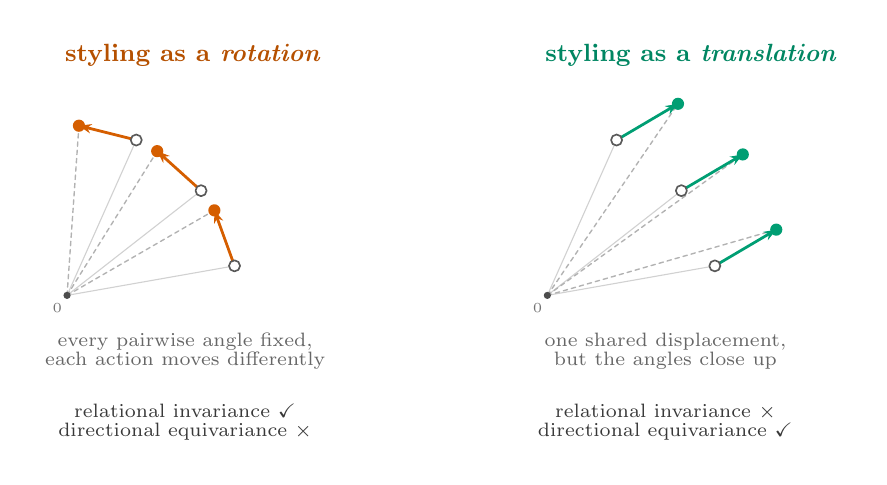
\begin{tikzpicture}[font=\small,line cap=round,line join=round,x=1cm,y=1cm]
\useasboundingbox (-0.5,-2.05) rectangle (10.05,3.4);
\begin{scope}[shift={(0.0,0)}]
\node[font=\small\bfseries,text=okverm!85!black,anchor=west] at (-0.15,3.05) {styling as a \emph{rotation}};
\draw[black!18,line width=0.4pt] (0,0) -- (2.127,0.375);
\draw[black!30,line width=0.5pt,dash pattern=on 1.6pt off 1.4pt] (0,0) -- (1.871,1.080);
\draw[-{Stealth[length=4.5pt,width=3.4pt]},okverm,line width=1.0pt] (2.127,0.375) -- (1.871,1.080);
\node[circle,draw=black!65,fill=white,inner sep=0pt,minimum size=4pt,line width=0.6pt] at (2.127,0.375) {};
\node[circle,fill=okverm,inner sep=0pt,minimum size=4.4pt] at (1.871,1.080) {};
\draw[black!18,line width=0.4pt] (0,0) -- (1.702,1.330);
\draw[black!30,line width=0.5pt,dash pattern=on 1.6pt off 1.4pt] (0,0) -- (1.145,1.832);
\draw[-{Stealth[length=4.5pt,width=3.4pt]},okverm,line width=1.0pt] (1.702,1.330) -- (1.145,1.832);
\node[circle,draw=black!65,fill=white,inner sep=0pt,minimum size=4pt,line width=0.6pt] at (1.702,1.330) {};
\node[circle,fill=okverm,inner sep=0pt,minimum size=4.4pt] at (1.145,1.832) {};
\draw[black!18,line width=0.4pt] (0,0) -- (0.879,1.973);
\draw[black!30,line width=0.5pt,dash pattern=on 1.6pt off 1.4pt] (0,0) -- (0.151,2.155);
\draw[-{Stealth[length=4.5pt,width=3.4pt]},okverm,line width=1.0pt] (0.879,1.973) -- (0.151,2.155);
\node[circle,draw=black!65,fill=white,inner sep=0pt,minimum size=4pt,line width=0.6pt] at (0.879,1.973) {};
\node[circle,fill=okverm,inner sep=0pt,minimum size=4.4pt] at (0.151,2.155) {};
\fill[black!70] (0,0) circle (1.3pt);
\node[font=\tiny,text=black!55,anchor=north east] at (0.06,0.02) {$0$};
\node[font=\scriptsize,text=black!60,align=center,anchor=north] at (1.5,-0.35) {every pairwise angle fixed,\\[-1pt] each action moves differently};
\node[font=\scriptsize,text=black!78,align=center,anchor=north] at (1.5,-1.25) {relational invariance \checkmark\\[-1pt] directional equivariance $\times$};
\end{scope}
\begin{scope}[shift={(6.1,0)}]
\node[font=\small\bfseries,text=okgreen!85!black,anchor=west] at (-0.15,3.05) {styling as a \emph{translation}};
\draw[black!18,line width=0.4pt] (0,0) -- (2.127,0.375);
\draw[black!30,line width=0.5pt,dash pattern=on 1.6pt off 1.4pt] (0,0) -- (2.907,0.835);
\draw[-{Stealth[length=4.5pt,width=3.4pt]},okgreen,line width=1.0pt] (2.127,0.375) -- (2.907,0.835);
\node[circle,draw=black!65,fill=white,inner sep=0pt,minimum size=4pt,line width=0.6pt] at (2.127,0.375) {};
\node[circle,fill=okgreen,inner sep=0pt,minimum size=4.4pt] at (2.907,0.835) {};
\draw[black!18,line width=0.4pt] (0,0) -- (1.702,1.330);
\draw[black!30,line width=0.5pt,dash pattern=on 1.6pt off 1.4pt] (0,0) -- (2.482,1.790);
\draw[-{Stealth[length=4.5pt,width=3.4pt]},okgreen,line width=1.0pt] (1.702,1.330) -- (2.482,1.790);
\node[circle,draw=black!65,fill=white,inner sep=0pt,minimum size=4pt,line width=0.6pt] at (1.702,1.330) {};
\node[circle,fill=okgreen,inner sep=0pt,minimum size=4.4pt] at (2.482,1.790) {};
\draw[black!18,line width=0.4pt] (0,0) -- (0.879,1.973);
\draw[black!30,line width=0.5pt,dash pattern=on 1.6pt off 1.4pt] (0,0) -- (1.659,2.433);
\draw[-{Stealth[length=4.5pt,width=3.4pt]},okgreen,line width=1.0pt] (0.879,1.973) -- (1.659,2.433);
\node[circle,draw=black!65,fill=white,inner sep=0pt,minimum size=4pt,line width=0.6pt] at (0.879,1.973) {};
\node[circle,fill=okgreen,inner sep=0pt,minimum size=4.4pt] at (1.659,2.433) {};
\fill[black!70] (0,0) circle (1.3pt);
\node[font=\tiny,text=black!55,anchor=north east] at (0.06,0.02) {$0$};
\node[font=\scriptsize,text=black!60,align=center,anchor=north] at (1.5,-0.35) {one shared displacement,\\[-1pt] but the angles close up};
\node[font=\scriptsize,text=black!78,align=center,anchor=north] at (1.5,-1.25) {relational invariance $\times$\\[-1pt] directional equivariance \checkmark};
\end{scope}
\end{tikzpicture}
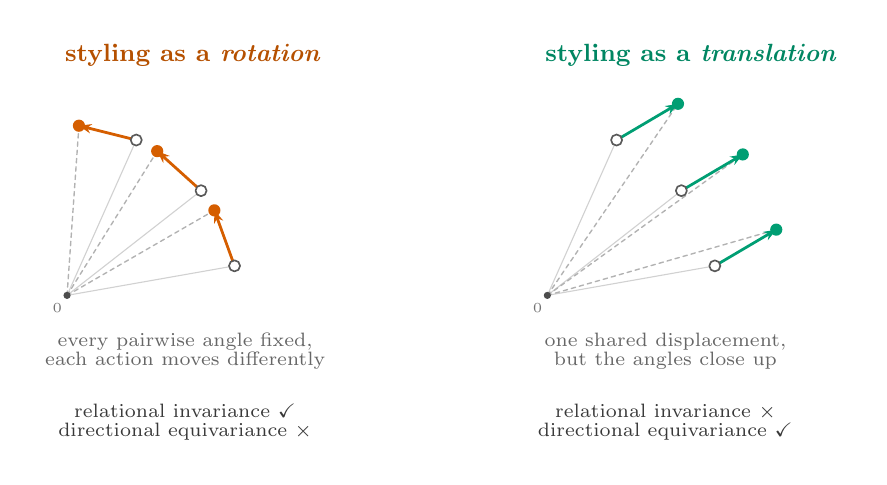
\begin{tikzpicture}[font=\small,line cap=round,line join=round,x=1cm,y=1cm]
\useasboundingbox (-0.5,-2.05) rectangle (10.05,3.4);
\begin{scope}[shift={(0.0,0)}]
\node[font=\small\bfseries,text=okverm!85!black,anchor=west] at (-0.15,3.05) {styling as a \emph{rotation}};
\draw[black!18,line width=0.4pt] (0,0) -- (2.127,0.375);
\draw[black!30,line width=0.5pt,dash pattern=on 1.6pt off 1.4pt] (0,0) -- (1.871,1.080);
\draw[-{Stealth[length=4.5pt,width=3.4pt]},okverm,line width=1.0pt] (2.127,0.375) -- (1.871,1.080);
\node[circle,draw=black!65,fill=white,inner sep=0pt,minimum size=4pt,line width=0.6pt] at (2.127,0.375) {};
\node[circle,fill=okverm,inner sep=0pt,minimum size=4.4pt] at (1.871,1.080) {};
\draw[black!18,line width=0.4pt] (0,0) -- (1.702,1.330);
\draw[black!30,line width=0.5pt,dash pattern=on 1.6pt off 1.4pt] (0,0) -- (1.145,1.832);
\draw[-{Stealth[length=4.5pt,width=3.4pt]},okverm,line width=1.0pt] (1.702,1.330) -- (1.145,1.832);
\node[circle,draw=black!65,fill=white,inner sep=0pt,minimum size=4pt,line width=0.6pt] at (1.702,1.330) {};
\node[circle,fill=okverm,inner sep=0pt,minimum size=4.4pt] at (1.145,1.832) {};
\draw[black!18,line width=0.4pt] (0,0) -- (0.879,1.973);
\draw[black!30,line width=0.5pt,dash pattern=on 1.6pt off 1.4pt] (0,0) -- (0.151,2.155);
\draw[-{Stealth[length=4.5pt,width=3.4pt]},okverm,line width=1.0pt] (0.879,1.973) -- (0.151,2.155);
\node[circle,draw=black!65,fill=white,inner sep=0pt,minimum size=4pt,line width=0.6pt] at (0.879,1.973) {};
\node[circle,fill=okverm,inner sep=0pt,minimum size=4.4pt] at (0.151,2.155) {};
\fill[black!70] (0,0) circle (1.3pt);
\node[font=\tiny,text=black!55,anchor=north east] at (0.06,0.02) {$0$};
\node[font=\scriptsize,text=black!60,align=center,anchor=north] at (1.5,-0.35) {every pairwise angle fixed,\\[-1pt] each action moves differently};
\node[font=\scriptsize,text=black!78,align=center,anchor=north] at (1.5,-1.25) {relational invariance \checkmark\\[-1pt] directional equivariance $\times$};
\end{scope}
\begin{scope}[shift={(6.1,0)}]
\node[font=\small\bfseries,text=okgreen!85!black,anchor=west] at (-0.15,3.05) {styling as a \emph{translation}};
\draw[black!18,line width=0.4pt] (0,0) -- (2.127,0.375);
\draw[black!30,line width=0.5pt,dash pattern=on 1.6pt off 1.4pt] (0,0) -- (2.907,0.835);
\draw[-{Stealth[length=4.5pt,width=3.4pt]},okgreen,line width=1.0pt] (2.127,0.375) -- (2.907,0.835);
\node[circle,draw=black!65,fill=white,inner sep=0pt,minimum size=4pt,line width=0.6pt] at (2.127,0.375) {};
\node[circle,fill=okgreen,inner sep=0pt,minimum size=4.4pt] at (2.907,0.835) {};
\draw[black!18,line width=0.4pt] (0,0) -- (1.702,1.330);
\draw[black!30,line width=0.5pt,dash pattern=on 1.6pt off 1.4pt] (0,0) -- (2.482,1.790);
\draw[-{Stealth[length=4.5pt,width=3.4pt]},okgreen,line width=1.0pt] (1.702,1.330) -- (2.482,1.790);
\node[circle,draw=black!65,fill=white,inner sep=0pt,minimum size=4pt,line width=0.6pt] at (1.702,1.330) {};
\node[circle,fill=okgreen,inner sep=0pt,minimum size=4.4pt] at (2.482,1.790) {};
\draw[black!18,line width=0.4pt] (0,0) -- (0.879,1.973);
\draw[black!30,line width=0.5pt,dash pattern=on 1.6pt off 1.4pt] (0,0) -- (1.659,2.433);
\draw[-{Stealth[length=4.5pt,width=3.4pt]},okgreen,line width=1.0pt] (0.879,1.973) -- (1.659,2.433);
\node[circle,draw=black!65,fill=white,inner sep=0pt,minimum size=4pt,line width=0.6pt] at (0.879,1.973) {};
\node[circle,fill=okgreen,inner sep=0pt,minimum size=4.4pt] at (1.659,2.433) {};
\fill[black!70] (0,0) circle (1.3pt);
\node[font=\tiny,text=black!55,anchor=north east] at (0.06,0.02) {$0$};
\node[font=\scriptsize,text=black!60,align=center,anchor=north] at (1.5,-0.35) {one shared displacement,\\[-1pt] but the angles close up};
\node[font=\scriptsize,text=black!78,align=center,anchor=north] at (1.5,-1.25) {relational invariance $\times$\\[-1pt] directional equivariance \checkmark};
\end{scope}
\end{tikzpicture}
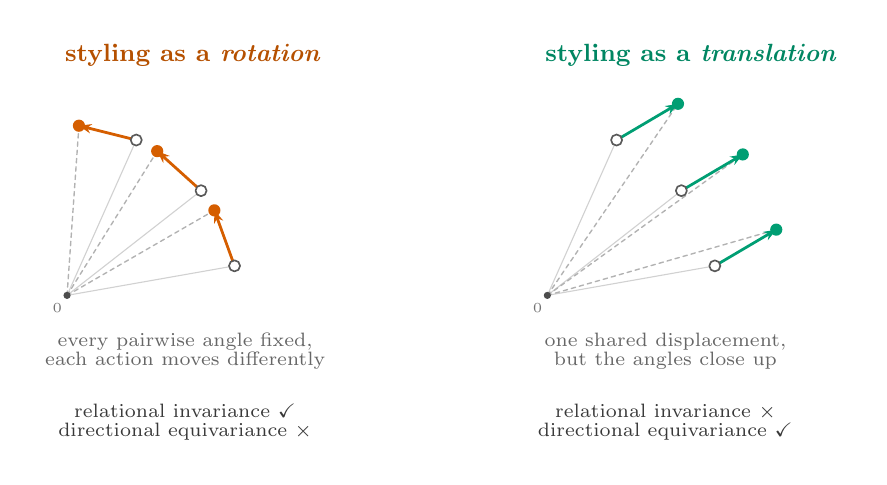
\begin{tikzpicture}[font=\small,line cap=round,line join=round,x=1cm,y=1cm]
\useasboundingbox (-0.5,-2.05) rectangle (10.05,3.4);
\begin{scope}[shift={(0.0,0)}]
\node[font=\small\bfseries,text=okverm!85!black,anchor=west] at (-0.15,3.05) {styling as a \emph{rotation}};
\draw[black!18,line width=0.4pt] (0,0) -- (2.127,0.375);
\draw[black!30,line width=0.5pt,dash pattern=on 1.6pt off 1.4pt] (0,0) -- (1.871,1.080);
\draw[-{Stealth[length=4.5pt,width=3.4pt]},okverm,line width=1.0pt] (2.127,0.375) -- (1.871,1.080);
\node[circle,draw=black!65,fill=white,inner sep=0pt,minimum size=4pt,line width=0.6pt] at (2.127,0.375) {};
\node[circle,fill=okverm,inner sep=0pt,minimum size=4.4pt] at (1.871,1.080) {};
\draw[black!18,line width=0.4pt] (0,0) -- (1.702,1.330);
\draw[black!30,line width=0.5pt,dash pattern=on 1.6pt off 1.4pt] (0,0) -- (1.145,1.832);
\draw[-{Stealth[length=4.5pt,width=3.4pt]},okverm,line width=1.0pt] (1.702,1.330) -- (1.145,1.832);
\node[circle,draw=black!65,fill=white,inner sep=0pt,minimum size=4pt,line width=0.6pt] at (1.702,1.330) {};
\node[circle,fill=okverm,inner sep=0pt,minimum size=4.4pt] at (1.145,1.832) {};
\draw[black!18,line width=0.4pt] (0,0) -- (0.879,1.973);
\draw[black!30,line width=0.5pt,dash pattern=on 1.6pt off 1.4pt] (0,0) -- (0.151,2.155);
\draw[-{Stealth[length=4.5pt,width=3.4pt]},okverm,line width=1.0pt] (0.879,1.973) -- (0.151,2.155);
\node[circle,draw=black!65,fill=white,inner sep=0pt,minimum size=4pt,line width=0.6pt] at (0.879,1.973) {};
\node[circle,fill=okverm,inner sep=0pt,minimum size=4.4pt] at (0.151,2.155) {};
\fill[black!70] (0,0) circle (1.3pt);
\node[font=\tiny,text=black!55,anchor=north east] at (0.06,0.02) {$0$};
\node[font=\scriptsize,text=black!60,align=center,anchor=north] at (1.5,-0.35) {every pairwise angle fixed,\\[-1pt] each action moves differently};
\node[font=\scriptsize,text=black!78,align=center,anchor=north] at (1.5,-1.25) {relational invariance \checkmark\\[-1pt] directional equivariance $\times$};
\end{scope}
\begin{scope}[shift={(6.1,0)}]
\node[font=\small\bfseries,text=okgreen!85!black,anchor=west] at (-0.15,3.05) {styling as a \emph{translation}};
\draw[black!18,line width=0.4pt] (0,0) -- (2.127,0.375);
\draw[black!30,line width=0.5pt,dash pattern=on 1.6pt off 1.4pt] (0,0) -- (2.907,0.835);
\draw[-{Stealth[length=4.5pt,width=3.4pt]},okgreen,line width=1.0pt] (2.127,0.375) -- (2.907,0.835);
\node[circle,draw=black!65,fill=white,inner sep=0pt,minimum size=4pt,line width=0.6pt] at (2.127,0.375) {};
\node[circle,fill=okgreen,inner sep=0pt,minimum size=4.4pt] at (2.907,0.835) {};
\draw[black!18,line width=0.4pt] (0,0) -- (1.702,1.330);
\draw[black!30,line width=0.5pt,dash pattern=on 1.6pt off 1.4pt] (0,0) -- (2.482,1.790);
\draw[-{Stealth[length=4.5pt,width=3.4pt]},okgreen,line width=1.0pt] (1.702,1.330) -- (2.482,1.790);
\node[circle,draw=black!65,fill=white,inner sep=0pt,minimum size=4pt,line width=0.6pt] at (1.702,1.330) {};
\node[circle,fill=okgreen,inner sep=0pt,minimum size=4.4pt] at (2.482,1.790) {};
\draw[black!18,line width=0.4pt] (0,0) -- (0.879,1.973);
\draw[black!30,line width=0.5pt,dash pattern=on 1.6pt off 1.4pt] (0,0) -- (1.659,2.433);
\draw[-{Stealth[length=4.5pt,width=3.4pt]},okgreen,line width=1.0pt] (0.879,1.973) -- (1.659,2.433);
\node[circle,draw=black!65,fill=white,inner sep=0pt,minimum size=4pt,line width=0.6pt] at (0.879,1.973) {};
\node[circle,fill=okgreen,inner sep=0pt,minimum size=4.4pt] at (1.659,2.433) {};
\fill[black!70] (0,0) circle (1.3pt);
\node[font=\tiny,text=black!55,anchor=north east] at (0.06,0.02) {$0$};
\node[font=\scriptsize,text=black!60,align=center,anchor=north] at (1.5,-0.35) {one shared displacement,\\[-1pt] but the angles close up};
\node[font=\scriptsize,text=black!78,align=center,anchor=north] at (1.5,-1.25) {relational invariance $\times$\\[-1pt] directional equivariance \checkmark};
\end{scope}
\end{tikzpicture}
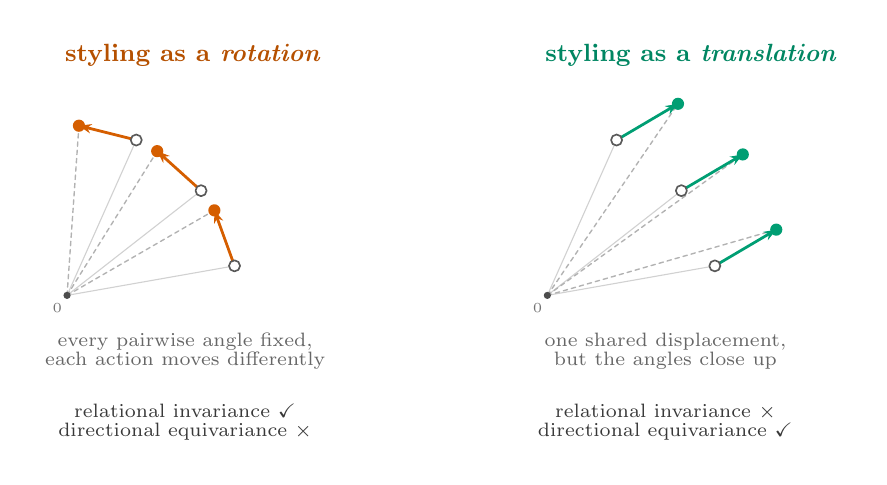
\begin{tikzpicture}[font=\small,line cap=round,line join=round,x=1cm,y=1cm]
\useasboundingbox (-0.5,-2.05) rectangle (10.05,3.4);
\begin{scope}[shift={(0.0,0)}]
\node[font=\small\bfseries,text=okverm!85!black,anchor=west] at (-0.15,3.05) {styling as a \emph{rotation}};
\draw[black!18,line width=0.4pt] (0,0) -- (2.127,0.375);
\draw[black!30,line width=0.5pt,dash pattern=on 1.6pt off 1.4pt] (0,0) -- (1.871,1.080);
\draw[-{Stealth[length=4.5pt,width=3.4pt]},okverm,line width=1.0pt] (2.127,0.375) -- (1.871,1.080);
\node[circle,draw=black!65,fill=white,inner sep=0pt,minimum size=4pt,line width=0.6pt] at (2.127,0.375) {};
\node[circle,fill=okverm,inner sep=0pt,minimum size=4.4pt] at (1.871,1.080) {};
\draw[black!18,line width=0.4pt] (0,0) -- (1.702,1.330);
\draw[black!30,line width=0.5pt,dash pattern=on 1.6pt off 1.4pt] (0,0) -- (1.145,1.832);
\draw[-{Stealth[length=4.5pt,width=3.4pt]},okverm,line width=1.0pt] (1.702,1.330) -- (1.145,1.832);
\node[circle,draw=black!65,fill=white,inner sep=0pt,minimum size=4pt,line width=0.6pt] at (1.702,1.330) {};
\node[circle,fill=okverm,inner sep=0pt,minimum size=4.4pt] at (1.145,1.832) {};
\draw[black!18,line width=0.4pt] (0,0) -- (0.879,1.973);
\draw[black!30,line width=0.5pt,dash pattern=on 1.6pt off 1.4pt] (0,0) -- (0.151,2.155);
\draw[-{Stealth[length=4.5pt,width=3.4pt]},okverm,line width=1.0pt] (0.879,1.973) -- (0.151,2.155);
\node[circle,draw=black!65,fill=white,inner sep=0pt,minimum size=4pt,line width=0.6pt] at (0.879,1.973) {};
\node[circle,fill=okverm,inner sep=0pt,minimum size=4.4pt] at (0.151,2.155) {};
\fill[black!70] (0,0) circle (1.3pt);
\node[font=\tiny,text=black!55,anchor=north east] at (0.06,0.02) {$0$};
\node[font=\scriptsize,text=black!60,align=center,anchor=north] at (1.5,-0.35) {every pairwise angle fixed,\\[-1pt] each action moves differently};
\node[font=\scriptsize,text=black!78,align=center,anchor=north] at (1.5,-1.25) {relational invariance \checkmark\\[-1pt] directional equivariance $\times$};
\end{scope}
\begin{scope}[shift={(6.1,0)}]
\node[font=\small\bfseries,text=okgreen!85!black,anchor=west] at (-0.15,3.05) {styling as a \emph{translation}};
\draw[black!18,line width=0.4pt] (0,0) -- (2.127,0.375);
\draw[black!30,line width=0.5pt,dash pattern=on 1.6pt off 1.4pt] (0,0) -- (2.907,0.835);
\draw[-{Stealth[length=4.5pt,width=3.4pt]},okgreen,line width=1.0pt] (2.127,0.375) -- (2.907,0.835);
\node[circle,draw=black!65,fill=white,inner sep=0pt,minimum size=4pt,line width=0.6pt] at (2.127,0.375) {};
\node[circle,fill=okgreen,inner sep=0pt,minimum size=4.4pt] at (2.907,0.835) {};
\draw[black!18,line width=0.4pt] (0,0) -- (1.702,1.330);
\draw[black!30,line width=0.5pt,dash pattern=on 1.6pt off 1.4pt] (0,0) -- (2.482,1.790);
\draw[-{Stealth[length=4.5pt,width=3.4pt]},okgreen,line width=1.0pt] (1.702,1.330) -- (2.482,1.790);
\node[circle,draw=black!65,fill=white,inner sep=0pt,minimum size=4pt,line width=0.6pt] at (1.702,1.330) {};
\node[circle,fill=okgreen,inner sep=0pt,minimum size=4.4pt] at (2.482,1.790) {};
\draw[black!18,line width=0.4pt] (0,0) -- (0.879,1.973);
\draw[black!30,line width=0.5pt,dash pattern=on 1.6pt off 1.4pt] (0,0) -- (1.659,2.433);
\draw[-{Stealth[length=4.5pt,width=3.4pt]},okgreen,line width=1.0pt] (0.879,1.973) -- (1.659,2.433);
\node[circle,draw=black!65,fill=white,inner sep=0pt,minimum size=4pt,line width=0.6pt] at (0.879,1.973) {};
\node[circle,fill=okgreen,inner sep=0pt,minimum size=4.4pt] at (1.659,2.433) {};
\fill[black!70] (0,0) circle (1.3pt);
\node[font=\tiny,text=black!55,anchor=north east] at (0.06,0.02) {$0$};
\node[font=\scriptsize,text=black!60,align=center,anchor=north] at (1.5,-0.35) {one shared displacement,\\[-1pt] but the angles close up};
\node[font=\scriptsize,text=black!78,align=center,anchor=north] at (1.5,-1.25) {relational invariance $\times$\\[-1pt] directional equivariance \checkmark};
\end{scope}
\end{tikzpicture}
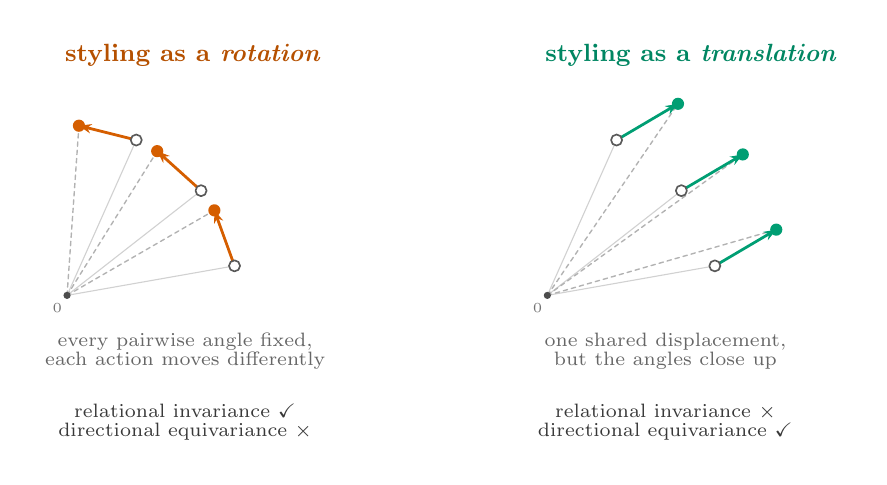
\begin{tikzpicture}[font=\small,line cap=round,line join=round,x=1cm,y=1cm]
\useasboundingbox (-0.5,-2.05) rectangle (10.05,3.4);
\begin{scope}[shift={(0.0,0)}]
\node[font=\small\bfseries,text=okverm!85!black,anchor=west] at (-0.15,3.05) {styling as a \emph{rotation}};
\draw[black!18,line width=0.4pt] (0,0) -- (2.127,0.375);
\draw[black!30,line width=0.5pt,dash pattern=on 1.6pt off 1.4pt] (0,0) -- (1.871,1.080);
\draw[-{Stealth[length=4.5pt,width=3.4pt]},okverm,line width=1.0pt] (2.127,0.375) -- (1.871,1.080);
\node[circle,draw=black!65,fill=white,inner sep=0pt,minimum size=4pt,line width=0.6pt] at (2.127,0.375) {};
\node[circle,fill=okverm,inner sep=0pt,minimum size=4.4pt] at (1.871,1.080) {};
\draw[black!18,line width=0.4pt] (0,0) -- (1.702,1.330);
\draw[black!30,line width=0.5pt,dash pattern=on 1.6pt off 1.4pt] (0,0) -- (1.145,1.832);
\draw[-{Stealth[length=4.5pt,width=3.4pt]},okverm,line width=1.0pt] (1.702,1.330) -- (1.145,1.832);
\node[circle,draw=black!65,fill=white,inner sep=0pt,minimum size=4pt,line width=0.6pt] at (1.702,1.330) {};
\node[circle,fill=okverm,inner sep=0pt,minimum size=4.4pt] at (1.145,1.832) {};
\draw[black!18,line width=0.4pt] (0,0) -- (0.879,1.973);
\draw[black!30,line width=0.5pt,dash pattern=on 1.6pt off 1.4pt] (0,0) -- (0.151,2.155);
\draw[-{Stealth[length=4.5pt,width=3.4pt]},okverm,line width=1.0pt] (0.879,1.973) -- (0.151,2.155);
\node[circle,draw=black!65,fill=white,inner sep=0pt,minimum size=4pt,line width=0.6pt] at (0.879,1.973) {};
\node[circle,fill=okverm,inner sep=0pt,minimum size=4.4pt] at (0.151,2.155) {};
\fill[black!70] (0,0) circle (1.3pt);
\node[font=\tiny,text=black!55,anchor=north east] at (0.06,0.02) {$0$};
\node[font=\scriptsize,text=black!60,align=center,anchor=north] at (1.5,-0.35) {every pairwise angle fixed,\\[-1pt] each action moves differently};
\node[font=\scriptsize,text=black!78,align=center,anchor=north] at (1.5,-1.25) {relational invariance \checkmark\\[-1pt] directional equivariance $\times$};
\end{scope}
\begin{scope}[shift={(6.1,0)}]
\node[font=\small\bfseries,text=okgreen!85!black,anchor=west] at (-0.15,3.05) {styling as a \emph{translation}};
\draw[black!18,line width=0.4pt] (0,0) -- (2.127,0.375);
\draw[black!30,line width=0.5pt,dash pattern=on 1.6pt off 1.4pt] (0,0) -- (2.907,0.835);
\draw[-{Stealth[length=4.5pt,width=3.4pt]},okgreen,line width=1.0pt] (2.127,0.375) -- (2.907,0.835);
\node[circle,draw=black!65,fill=white,inner sep=0pt,minimum size=4pt,line width=0.6pt] at (2.127,0.375) {};
\node[circle,fill=okgreen,inner sep=0pt,minimum size=4.4pt] at (2.907,0.835) {};
\draw[black!18,line width=0.4pt] (0,0) -- (1.702,1.330);
\draw[black!30,line width=0.5pt,dash pattern=on 1.6pt off 1.4pt] (0,0) -- (2.482,1.790);
\draw[-{Stealth[length=4.5pt,width=3.4pt]},okgreen,line width=1.0pt] (1.702,1.330) -- (2.482,1.790);
\node[circle,draw=black!65,fill=white,inner sep=0pt,minimum size=4pt,line width=0.6pt] at (1.702,1.330) {};
\node[circle,fill=okgreen,inner sep=0pt,minimum size=4.4pt] at (2.482,1.790) {};
\draw[black!18,line width=0.4pt] (0,0) -- (0.879,1.973);
\draw[black!30,line width=0.5pt,dash pattern=on 1.6pt off 1.4pt] (0,0) -- (1.659,2.433);
\draw[-{Stealth[length=4.5pt,width=3.4pt]},okgreen,line width=1.0pt] (0.879,1.973) -- (1.659,2.433);
\node[circle,draw=black!65,fill=white,inner sep=0pt,minimum size=4pt,line width=0.6pt] at (0.879,1.973) {};
\node[circle,fill=okgreen,inner sep=0pt,minimum size=4.4pt] at (1.659,2.433) {};
\fill[black!70] (0,0) circle (1.3pt);
\node[font=\tiny,text=black!55,anchor=north east] at (0.06,0.02) {$0$};
\node[font=\scriptsize,text=black!60,align=center,anchor=north] at (1.5,-0.35) {one shared displacement,\\[-1pt] but the angles close up};
\node[font=\scriptsize,text=black!78,align=center,anchor=north] at (1.5,-1.25) {relational invariance $\times$\\[-1pt] directional equivariance \checkmark};
\end{scope}
\end{tikzpicture}
\end{document}
